 \chapter{Découverte des circonstances factuelles par regroupement non supervisé de documents}
\label{chap:similarite}

\section{Introduction}
\label{sec:similarite:introduction}
Les circonstances factuelles définissent les contextes possibles dans lesquels une catégorie de demande peut être formulée (voir \ref{sec:similarite:données} pour des exemples). Les analyses descriptives ou prédictives ne prennent sens que lorsqu'elles sont appliquées à un ensemble de décisions aux circonstances similaires. Par exemple, il serait imprudent de considérer toutes les décisions pour analyser les chances d'acceptation d'une demande de dommages et intérêts fondée sur l'\og article 700 du code de procédure civile \fg{}. Les taux d'acceptation ou de rejet peuvent être différents entre des affaires de licenciement et celles portant sur les troubles anormaux du voisinage, et même plus spécifiquement entre les troubles de voisinage entre particulier et entreprises. % (par exemple: chantier de construction), ou simplement entre particuliers (par exemple: troubles sonores). 
 Il serait préférable de travailler uniquement avec des décisions similaires à la situation d'intérêt. L'identification des circonstances factuelles devient donc une étape préalable indispensable à l'analyse du résultat. Malheureusement, les circonstances sont très diverses et quasi infinies pour être identifiées par classification supervisée à l'aide d'annotation manuelle d'exemples comme dans les chapitres précédents. Il est donc plus adéquat d'adopter une approche non-supervisée capable de découvrir les circonstances factuelles à partir d'un corpus de documents d'une même catégorie de demande. Plus précisément, la méthode doit construire des sous-ensembles de décisions partageant des situations similaires.  L'objectif de ce chapitre est d'expérimenter des algorithmes  de regroupement (\textit{clustering}) et des métriques de similarité généralement utilisées sur les textes. Ce chapitre propose aussi une méthode d'apprentissage d'une distance qui est basée sur la transformation de documents, et montre qu'une telle métrique permet de bien mesurer la (dis-) similarité sémantique définie par les circonstances factuelles.

%\section{Formulation du Problème}
%\label{sec:similarite:probleme}

\section{Catégorisation non-supervisée de documents}
\label{sec:similarite:biblio}

Cette section fait une synthèse bibliographique de différents aspects qui rentrent dans la conception d'un système de regroupement de documents. Elle aborde principalement le choix de l'algorithme, la définition d'une mesure de similarité, la représentation des documents, la détermination du nombre de groupes (appelés \textit{clusters}), et l'évaluation de la catégorisation générée. Le corpus à catégoriser est noté $\mathcal{D}$ et comprend $N$ documents. Tout document $d \in \mathcal{D}$ est une séquence de mots $d=(d[1], \dots, d[\setsize{d}])$, où $d_i$ est le mot à la position $i$ dans $d$. Sa représentation vectorielle  est notée $\vec{d}=(\vec{d}[1], \vec{d}[2], \dots, \vec{d}[m])$. Pour un modèle vectoriel de type TF-IDF de vocabulaire $T = \lbrace t_1, t_2, \dots, t_m \rbrace$, $\vec{d}[i] = w(t_i,d)$ est le poids du terme $t_i \in T$ dans le texte $d$ ({cf. \ref{sec:quanta:classification}}). La catégorisation obtenue est un ensemble de clusters $C = \lbrace C_1, C_2, \cdots, C_K \rbrace$, $K$ étant le nombre de clusters formés.

\subsection{Algorithmes de catégorisation non-supervisé}

La catégorisation de documents a pour objectif  d'identifier, sans supervision\footnote{Sans utiliser des exemples annotés.}, une organisation pertinente (pour le domaine expert) dans l'ensemble $\mathcal{D}$ en construisant des groupes représentants des catégories inconnues au départ. Ces groupes, appelés clusters, peuvent être disjoints ou se chevaucher, et plates ou hiérarchiques suivant les contraintes du domaine expert. L’algorithme à utiliser dépend généralement de la forme qu’on souhaite donner à l’organisation. 

\subsubsection{Partitionnement disjoint}
Pour réaliser des partitions distinctes\footnote{Chaque document n'appartient qu'à un seul cluster.} (\textit{hard clustering}), des algorithmes tels que celui des K-moyennes (\textit{K-means}) \citep{forgey1965kmeans} et celui des K-medoïdes (\textit{K-medoids}) \citep{kaufman1987kmedoids} sont les plus simples \citep{balabantaray2015KmeansKmedoids}. Ces deux algorithmes fonctionnent de manière similaire, et nécessitent que le nombre $K$ de clusters soient prédéfini. Ils commencent par une définition aléatoire de $K$ centres initiaux de clusters (\textit{centroïdes}) et l'affectation des différents documents au cluster dont le centre est le plus proche. S'en suit une boucle dans laquelle le centroïde est recalculé (le point dont la somme des distances aux membres du cluster est minimale) et les documents sont réaffectés chacun au cluster dont le centroïde est le plus proche. L'algorithme s'arrête si aucune amélioration n'est plus observée, ce qui se traduit soit par l'atteinte d'une valeur minimale prédéfinie de l'erreur de catégorisation\footnote{Somme des distances au carré entre les points et leur centre respectif.} ou d'une mesure d'évaluation non supervisée (\ref{sec:similarite:biblio:unsupeval}). La différence entre l'algorithmes des K-moyennes et celui des K-medoïdes tient principalement au fait que les centroïdes du premier ne sont pas nécessairement des points (documents) de l'ensemble d'origine, mais des points moyennes des représentations vectorielles des membres du cluster, contrairement à l'algorithme des K-medoïdes qui ne considère comme centres que des documents de $\mathcal{D}$. Cette différence donne l'avantage au K-medoïdes de ne pas dépendre d'une représentation vectorielle nécessaire au calcul de la moyenne, mais elle a aussi l'inconvénient d'augmenter sa complexité en temps et en espace car il faut calculer et stocker la distance entre toutes les paires de documents. Il existe plusieurs autres algorithmes de partitionnement dont le principe est différent de celui des K-moyennes. Par exemple, l'algorithme DBSCAN (\textit{Density-based spatial clustering of applications with noise}) \citep{ester1996dbscan}  ne prend pas en paramètre le nombre de clusters à construire. Il est défini sur le concept de régions de densité caractérisées par la distance minimale $\epsilon$ autorisée entre deux points d'une même région, et le nombre maximal de points qui doivent être dans le voisinage de rayon $\epsilon$ d'un point pour que ce voisinage soit une région de densité (le point central est appelé "point noyau" (\textit{core point}). Le principe du DBSCAN est de construire les clusters successivement en reliant les régions (voisinages) dont les noyaux sont à distance plus ou moins inférieure à $\epsilon$. Les points qui sont seuls dans leur cluster sont qualifiés de points aberrants (\textit{outliers}). 
% amélioration par réduction de dimension

La catégorisation spectrale est une autre méthode efficace de partitionnement qui effectue préalablement une réduction de dimensions à l'aide du spectre\footnote{Le spectre d'une matrice est l'ensemble de ses valeurs propres} de la matrice de similarité $M \in \mathbb{R}^{N \times N}$ \footnote{$M_{ij}$ est la mesure de la similarité entre les élément $d_i$ et $d_j$ de $\mathcal{D}$.} des données  avant d'appliquer un algorithme traditionnel comme celui des K-moyennes. Les dimensions du nouvel espace sont définies par les vecteurs propres de la matrice Laplacienne $L$ de $M$ \citep{shi2000spectralClustering, von2007tutorialSpectralClustering} qui peut être normalisée ($L = T^{-1/2}(T-S)T{-1/2}$) ou pas ($L = T - M$), $T$ étant la matrice diagonale déduite de $M$ i.e. $T_{ii} = \sum\limits_j M_{ij}$. 

Il est aussi possible d'utiliser les arbres de décision pour améliorer les résultats des K-moyennes. En effet, les forêts aléatoires \citep{breiman2001randomforest} permettent d'estimer la similarité entre deux points. Le principe consiste à générer un ensemble de $n$ points synthétiques, et d'entraîner une forêt aléatoire à une classification binaire supervisée avec les points originaux considérés dans la classe des "originaux" et les données synthétiques dans la seconde classe des "synthétiques" \citep{afanador2016unsupervisedrandomforest}. %Étant un ensemble d'arbre de décisions, % quel type d'arbre est utilisé pour le clustering de l'expérimentation?
une forêt aléatoire construit des arbres de décision sur des parties de l'ensemble d'apprentissage, auxquelles on a retiré une ou plusieurs variables prédictives. La similarité entre 2 points est la proportion d'arbres dans lesquels ces points se trouvent dans le même nœud feuille. Cette métrique "apprise" peut-être par la suite utilisée dans un algorithme comme les K-moyennes.

%\textcolor{red}{Random Forest - processus de construction: \url{https://onlinelibrary.wiley.com/doi/pdf/10.1002/cem.2790}}

%L'application de ces différents algorithmes aux documents n'est généralement basé que sur les statistiques d'occurrence des termes, et par conséquent les thématiques abordées dans les documents ne sont pas bien prise en compte, surtout que l'élimination des \og mots vides \fg{} (\textit{stop words}) peut laisser les deux documents sans sinon très peu de mots en commun \cite{kusner2015wordmoverdist}. \citet{xie2013MGCTM} démontrent empiriquement que l'intégration de la  modélisation thématique (\textit{topic modeling}) au clustering de documents améliore significativement les résultats. Cette intégration des modèles thématiques dans le clustering de documents peut être réalisée de multiples façons, mais deux méthodes semblent être les plus efficaces:
%\begin{enumerate}
%	\item l'intégration naïve \citep{lu2011K-moyennesLDApLSA} qui consiste à inférer $K$ thèmes à l'aide d'un algorithme comme le PLSA (aAnalyse sémantique probabiliste latente) \citep{hofmann1999PLSA} ou le LDA (allocation de Dirichlet latente)\citep{blei2003lda}, puis de considérer pour chaque document le thème $j \in [1..K]$ qui a la probabilité $\theta_j$ la plus élevé dans ce document suivant la distribution $\theta$ de probabilité des thèmes dans ce document; le thème choisi $j$ représente le cluster du document;
%	\item le modèle thématique multi-grain de clustering (\textit{multi-grain clustering topic model}) ou MGCTM proposé par \citet{xie2013MGCTM}, dont l'objectif est d'inférer de manière jointe les clusters et le modèle thématique.
%\end{enumerate}

\subsubsection{Catégorisation avec chevauchements}

Lorsque des chevauchements sont observables entre clusters\footnote{Un chevauchement est l'appartenance d'un document à plusieurs groupes}, un degré d'appartenance (\textit{membership degree}) d'un document à un chaque groupe est estimé par une fonction $u_{ij}, \forall d_i \in \mathcal{D}, \forall j \in [1..K]$  \citep{baraldi1999surveyfuzzyclstering}. Ce degré d'appartenance est employé dans des algorithmes de partitionnement "mou" comme l'algorithme des c-moyennes flou (FCM) \citep{bezdek1984fcm, hathaway1989fuzzycmeans}, ou le fuzzy c-Medoids (FDMdd) \citep{krishnapuram2001fuzzycmedoids}, ou la version améliorée IFKM (\textit{improved fuzzy K-medoids})\citep{sabzi2011fuzzykmedoids}.  Ces algorithmes consistent en deux étapes principales \citep{sabzi2011fuzzykmedoids}: 

\begin{enumerate}
 \item l'estimation des degrés d'appartenance de chaque instance $d_i \in \mathcal{D}$ à chaque cluster $j \in [1..K]$ de centroïde $z_j$ est réalisée par la minimisation de la fonction objective $P(\mathcal{D},Z) = \sum\limits_{i=1}^{n}\sum\limits_{j=1}^{k} \left[u_{ij}r(d_i,z_j)\right]$ \citep{krishnapuram2001fuzzycmedoids}  améliorée par \citet{sabzi2011fuzzykmedoids} en:
 \[P(\mathcal{D},Z) = \sum\limits_{i=1}^{N}\sum\limits_{j=1}^{K} \left[u_{ij}r(d_i,z_j)\right] + \lambda \sum\limits_{i=1}^{N}\sum\limits_{j=1}^{K} \left[ u_{ij}\log_2(u_{ij}) \right] \]
 \[s.c. \sum\limits_{j=1}^{k} u_{ij} = 1, 0 \leq u_{ij} < 1\]
 
 dont la valeur approximative de la solution est $u_{ij} = \frac{\exp\left(\frac{-r(d_i,z_j)}{\lambda}\right)}{\sum_{l=1}^{k}\exp\left(\frac{-r(d_l,z_j)}{\lambda}\right)},$ $r(d_i,z_j)$ étant la distance entre $d_i$ et  $z_j$;
 \item Le nouveau centre de chaque cluster est redéfini comme étant la moyenne des membres de chaque cluster chez le FCM. Mais pour les K-medoids flous, il s'agit le membre $z_j=d_i$ dont la somme des distances pondérées \footnote{la distance est pondérées par le degré d'appartenance de l'autre membre.} aux autres membres  est minimale: $\forall j \in  \left[1\twodots k \right]$, $z_j = \argmin\limits_{1 \leq q < s_j} \sum\limits_{i=1}^{s_j} \left[u_{ij}r(d_i,d_q)\right]$, $s_j$ étant la taille du cluster $j$.
\end{enumerate}
 Ainsi l'objectif de l'entraînement des algorithmes de catégorisation floue est double: déterminer les degrés optimaux d'appartenance $u_{ij}$ et l'ensemble $Z$ des centroïdes. \citet{nefti2004probabilisticFuzzyCMeans} proposent les C-moyennes floues probabilistes qui sont une variante du FCM pour laquelle la somme des degrés d'appartenance  d'un document aux clusters est de 1.
 
 Les regroupements avec chevauchement sont intéressants parce qu'il est possible qu'une décision traite de plusieurs circonstances factuelles.
%\textcolor{red}{A COMPLETER!!!!!!!!!!}
%Pour des regroupements hiérarchiques, des algorithmes comme celui du clustering par agglomération (\textit{agglomeration clustering}) sont mieux indiqués. Le principe du clustering par agglomération est de ...
%si les chevauchements sont négligeables ou n'existent pas, ou bien si la structure hiérarchique permettrait de mieux expliquer et distinguer les différences inter-groupes et les ressemblances intra-groupes. Nous souhaitons organiser des décisions de justices en fonction des circonstances factuelles auxquelles ces documents sont liés.  On pourrait par exemple faire une restriction des données aux cas où chaque document n’appartient qu’à une classe et proposer un système de clustering disjoint.

%\subsubsection{Limites des algorithmes de clustering}
%nombre prédéfini de clusters, initialisation aléatoire des centroïdes menant à des clusters différents entre plusieurs exécution \citep{sabzi2011fuzzyK-medoïdes}. Nous noterons aussi la dépendance à la métrique de similarité.
%Algorithme K-moyennes + kmédoids pour les documents: https://pdfs.semanticscholar.org/a46f/efdb64a01d1e6390c8212d881b9c4414ffbf.pdf

\subsubsection{Catégorisation hiérarchique}
La catégorisation hiérarchique consiste à construire une hiérarchie de clusters. Le regroupement hiérarchique ascendant ou regroupement \textit{agglomératif} (\textit{Agglomerative Clustering}) est une technique de catégorisation hiérarchique qui commence par autant de clusters que de documents (chacun des groupes comprenant un document). Ensuite, l'algorithme détecte et fusionne successivement les paires de groupes dont la fusion vérifie un critère (par exemple la paire est celle dont la distance est la plus petite et/ou proche d'une valeur seuil donnée, ou bien la fusion forme un groupe à inertie\footnote{L'inertie d'un cluster est la variance de ses points c'est-à-dire la somme des erreurs (distance d'un membre au centre) au carré.}minimale),
jusqu'à ce que tous les documents soient dans un unique groupe (racine). Pour déterminer le partitionnement optimal, le nombre de clusters doit être déterminé par l'une des diverses techniques existantes \citep{thorndike1953HAC_nb_clusters, salvador2004Hierarchical_clustering_number_of_clusters}.

\subsection{Métriques de dis-similarité (distances)}
\label{sec:similarite:distances}
Les algorithmes de catégorisation dépendent de la distance utilisée qui doit être bien choisie pour que le résultat révèlent au mieux la sémantique visée.
 Une métrique de dis-similarité $Dis$ est une fonction réelle d'une paire de documents $(d,d')$ qui mesure le degré de dis-similarité entre $d$ et $d'$  en satisfaisant aux propriétés suivantes $\forall d,d',d'' \in \mathcal{D}$ \citep{wang2015distancemetriclearningsurvey}:
\begin{enumerate}
\item $Dis(d,d') \geq 0$ ("non-négativité")
\item $Dis(d,d') = 0  \Leftrightarrow d = d'$ (identité discernable)
\item $Dis(d,d') = Dis(d', d)$ (symétrie)
\item $Dis(d,d'') \leq Dis(d,d') + Dis(d',d'')$ (inégalité triangulaire) \label{enum:sim:ineq-tri}
\end{enumerate}


La métrique peut être normée ($\forall (d,d') \in \mathcal{D} \times \mathcal{D};  0 \leq Dis(d,d') \leq 1$), à l'instar de la distance de Jaccard. Dans ce cas, la relation entre la similarité $Sim$ et la dis-similarité $Dis$ est définie par $Sim(d,d') = 1 - Dis(d,d')$.
%On parle de \textbf{pseudo-métrique} lorsque la condition \ref{enum:sim:ineq-tri} n'est pas satisfaite.

 Parmi les nombreuses métriques généralement utilisées  sur les textes \citep{huang2008similarityTextClustering, vijaymeena2016surveySim, afzali2018Simkmeans}, on retrouve par exemple:
\begin{itemize}
	\item Les distances de Minkowski {\footnotesize $Dis(d,d') = \norm{\vec{d} - \vec{d'}}_{Lp} = \sqrt[p]{\sum\limits_{i=1}^m \vert \vec{d}[i] - \vec{d}[i] \vert ^p}$}, dont font partie la distance euclidienne $Dis_{euclidienne}$ ($p=2$) et la distance de Manhattan $Dis_{manhattan}$ ($p=1$).
	%\item L'indice de Dice définit la similarité entre $d$ et $d'$ comme étant la proportion de termes qui leur sont communs: $Sim_{dice}(d,d') = \frac{2 \setsize{d \cap d'}}{\setsize{d} + \setsize{d'}}$.
	\item La distance de \citet{bray1957distance-braycurtis}: $Dis_{braycurtis}(d,d') = \frac{\sum\limits_{i=1}^m \vert \vec{d}[i] - \vec{d'}[i] \vert}{\sum\limits_{i=1}^m \vert \vec{d}[i] + \vec{d'}[i] \vert}$ \citep{huang2008similarityTextClustering}.
	\item La similarité cosinus est basée sur le cosinus de l'angle entre $\vec{d}$ et $\vec{d'}$ par la formule: $Sim_{cos}(d,d') = \frac{\vec{d}^t\vec{d'}}{\norm{\vec{d}}\norm{\vec{d'}}}$.
	Pour un modèle vectoriel du type TF-IDF, cette formulation considère que tous les termes du vocabulaire $T$ sont différents et ne partagent aucune relation. \citet{sidorov2014softcosine} la corrigent en proposant la fonction \textit{soft-cosine} utilisant la matrice de similarité entre  termes $S=\lbrace s_{ij}\rbrace_{1\leq i,j \leq m}$: 
	
	$Sim_{soft-cos}(d,d')= \frac{{\vec{d}}^T\cdot S\cdot \vec{d'}}{\sqrt{{\vec{d}}^T\cdot S\cdot \vec{d'}}\cdot \sqrt{\vec{d'}^T\cdot S\cdot \vec{d'}}} = \frac{\sum\limits_{1\leq i,j \leq m}s_{ij}\vec{d}[i]\vec{d'}[j]}{\sqrt{\sum\limits_{1\leq i,j \leq m}s_{ij}\vec{d}[i]\vec{d}[j]}\sqrt{\sum\limits_{1\leq i,j \leq m}s_{ij}\vec{d'}[i]\vec{d'}[j]}}$.
	
	$S$ peut être calculée à partir de n'importe quelle métrique comme la distance d'édition de Levenshtein (similarité lexicale) \citep{sidorov2014softcosine},  la similarité cosinus entre  plongements lexicaux \citep{charlet2017simbow_acl, charlet2018simbow_coria}, ou la similarité WordNet. La fonction cosinus  étant comprise entre -1 et +1, la distance déduite $Dis_{cos}(d,d') = 1 - Sim_{cos}(d,d')$ est comprise entre 1 et 2.
	
	\item Le coefficient similarité de \cite{jaccard1901similarite-jaccard}: {\footnotesize$Sim_{Jaccard}(d,d') = \frac{\vec{d}^T\vec{d'}}{\norm{\vec{d}}^2+\norm{\vec{d'}}^2 - \vec{d}^T\vec{d'}}$} \citep{huang2008similarityTextClustering} qui donne la distance {\footnotesize$Dis_{jaccard}(d,d') = 1-Sim(d,d')$}.
	%\item Le coefficient similarité de Dice: $Sim_{Dice}(x,x') = \frac{2\cdot \vert tok(x) \cap tok(x') \vert}{\vert tok(x) \vert + \vert tok(x')} $
	\item La similarité basée sur le coefficient de corrélation de Pearson est calculée comme suit \citep{huang2008similarityTextClustering}:
	
	{\footnotesize $Sim_{pearson}(d,d') = \frac{ \sum\limits^m_{i=1} \vec{d}[i] \cdot \vec{d'}[i] - TF_d\cdot TF_{d'}}{\sqrt{[m \sum\limits^m_{i=1} \vec{d}[i]^2 - TF^2_d][m \sum\limits^m_{i=1} \vec{d'}[i]^2 - TF^2_{d'}]}}$}, 
avec $TF_d = \sum\limits^m_{i=1} \vec{d}[i]$. Sa distance est déduite par la formule:

{\footnotesize $Dis_{pearson}(d,d') =
\left\{ \begin{array}{ll}
1 - Sim_{pearson}(d,d') & \text{si } Sim_{pearson}(d,d') \geq 0 \\
\vert Sim_{pearson}(d,d') \vert & \text{si } Sim_{pearson}(d,d') < 0.
\end{array}
\right.$}
%	\item Distance de la divergence moyenne de Kullback-Leibler considère un document comme une distribution de probabilité de termes, et mesure donc la similarité entre deux distributions: 
%	\[Dis_{avgKL}(x,x') = \sum\limits_{i=1}^m\big(\pi_1 \cdot D(w(t_i,x) \vert\vert w_t) + \pi_2 \cdot D(w(t_i,x') \vert\vert w_t) \big)\]
%	avec $\pi_1 = \frac{w(t_i,x)}{w(t_i,x) + w(t_i,x')}$, $\pi_2 = \frac{w(t_i,x')}{w(t_i,x) + w(t_i,x')}$, $D(a \vert\vert b) = a\cdot  \log_2(\frac{a}{b})$, et $w_t = \pi_1 \cdot w(t_i,x) + \pi_2 \cdot w(t_i,x')$
%	\item Okapi BM25 est une métrique de similarité généralement utilisée en recherche d'information pour calculer un score de pertinence d'un document D par rapport à une requête Q: 
%	\[Sim_{BM25}(Q,D) = \sum\limits_{w \in Q \cap D} \left( \frac{(k_3+1) \cdot c(w, Q)}{k_3 + c(w, Q)} \cdot f(w,D) \cdot \log \frac{N+1}{df(w) + 0.5)}\right),\]
%	\[\text{avec } f(w,D) = \frac{(k_1+1)\cdot c(w,D)}{k_1(1-b+b\frac{\vert D \vert}{avgdl})} = \frac{(k_1+1)\cdot c'(w,D)}{k_1 + c'(w,D)},\] où $c'(w,D) = \frac{c(w,D)}{1-b+b\frac{\vert D \vert}{avgdl} }$. $c'(w,D)$ pouvant approcher 0 pour des documents très longs, \citet{Lv2011BM25L} propose BM25L, une formulation plus robuste à la longueur des documents obtenue en remplaçant $f(w,D)$ par :
%	\[
%	f'(w,D) =
%	\left\{ \begin{array}{ll}
%	\frac{(k_1+1)\cdot (c'(q,D)+\delta)}{k_1+ (c'(w,D) + \delta)} & \text{si } c'(w,D) > 0 \\
%	0 & \text{si } sinon
%	\end{array}
%	\right.
%	\]
	\item \og La distance du déménageur de mot \fg{} (\textit{word mover's distance - WMD}) \citep{kusner2015wordmoverdist} est inclut la similarité sémantique entre les mots dans l'estimation de la distance entre documents. En effet, elle est la solution optimale du problème de transport suivant \footnote{Valeur minimale du cout cumulatif pondéré nécessaire pour déplacer  tous les mots de $d$ à $d'$ i.e. transformer $d$ en $d'$.}:
	
	\begin{equation*}\small
	\begin{aligned}
Dis_{wmd}(d, d') = 	& \min\limits_{T>0}
	& & \sum\limits_{i,j=1}^m T_{ij} c(i,j) \\
	& \text{s.c.}
	& & \sum\limits_{j=1}^m T_{ij} = \vec{d}[i], \forall i \in [1\twodots m];  \sum\limits_{i=1}^m T_{ij} = \vec{d'}[j], \forall j \in [1\twodots m]
	\end{aligned}
	\end{equation*} 
	
	$m$ est le nombre de mots considérés; $T$ est une matrice dont $T_{ij}$ est interprété comme étant la quantité du mot $i$ de $d$ qui est va au mot $j$ dans $d'$ ("voyage"). $c(i,j)$ est la distance euclidienne entre les vecteurs des mots $i$ et $j$; $\vec{d}[i] = \frac{compte(i, d)}{\sum\limits_{k=1}^m compte(k, d)}$, $compte(i, d)$ étant le nombre d'occurrences du mot $i$ dans $d$.
	
\end{itemize}


%Par contre, les métriques {apprises} sont définies à partir de connaissances des données labellisées. Ces métriques sont apprises pour répondre à la difficulté d'identifier la métrique statique appropriée pour un problème. L'apprentissage exploite un corpus préalablement annoté. L'apprentissage peut être supervisé si l'annotation du corpus consiste soit en classifiant des documents\footnote{Organisation des documents d'entraînement en des groupes aux labels prédéfinis.} \citep{weinberger2005LMNN}, soit en affectant des mesures de similarité à des paires de documents \citep{bibid}.  Un apprentissage semi-supervisé typique utilise des données annotées par jugements relatifs sur des pairs ou triplets de documents. Les contraintes de couples consistent en deux ensembles, l'un comprenant des couples de documents qui doivent être similaires, et l'autre contenant des couples de documents dis-similaires. Les contraintes de triplets consistent à définir pour un triplet de documents $(x_1,x_2,x_3)$ une comparaison de degré de similarité entre les paires (par exemple, $x_1$ est plus similaire à $x_2$ qu'à $x_3$). La métrique apprise est néanmoins une véritable métrique à valeur réelle positive écrite sous la forme d'une distance de Mahalanobis $f(x,y) = \sqrt{(x-y)^T M^{-1}(x-y)}$ (où $M$ est la matrice à apprendre). 
 
% L'apprentissage expérimenté dans ce chapitre est supervisé, même s'il utilise des données synthétiques. Nous supposons étant donné que les documents du corpus à \textit{clusteriser} sont tous de la même catégorie de demande, la différence entre les clusters et leur homogénéité se remarquera au niveau des faits. Par cette hypothèse, il reste un risque que d'autres types de regroupements se forment comme par exemple suivant d'autres catégories de demande co-occurrentes. Parmi les divers algorithmes réalisant un apprentissage supervisé, notons par exemple:
% \begin{itemize}
% 	\item Les plus-proches-voisins-dans-la-large-marge (LMNN) \citep{weinberger2005LMNN} plus adapté à l'annotation par classification;
% 	\item L'analyse des composants du voisinage (NCA) \citep{goldberger2005NCA};
% 	\item L'apprentissage de métrique pour la régression noyau (\textit{MLKR}) \citep{weinberger2007MLKR};
% 	\item L'analyse discriminante locale de Fisher (LFDA) \citep{sugiyama2007LFDA, } méthode supervisée (données labellisées) de réduction de dimension
% \end{itemize}

%@inproceedings{lemikolov2014word2vec,
%	title={Distributed representations of sentences and documents},
%	author={Le, Quoc and Mikolov, Tomas},
%	booktitle={International Conference on Machine Learning},
%	pages={1188--1196},
%	year={2014}
%}



\subsection{Représentation des textes}
\label{sec:similarite:representation}
\subsubsection{Modèle vectoriel}
La formulation des distances (cf.  \ref{sec:similarite:distances}) s'applique généralement à une représentation vectorielle des textes. Le chapitre \ref{chap:quanta} décrit différentes métriques de pondération des termes qui permettent de définir des variantes du modèle TF-IDF. Cependant, il s'agit de modèles basés uniquement sur le lexique des textes, et par conséquent, les distances appliquées sur ces représentations  correspondent à une similarité plus lexicale que sémantique. Il existe quelques techniques permettant de définir des dimensions par des thématiques qui transparaissent dans le corpus, et apportant par conséquent plus de sémantique à la représentation vectorielle.

\subsubsection{Réduction de dimension}
\label{sec:similarite:reduction-dimension}
La réduction de dimension a généralement pour but de réduire la taille de la représentation de documents i.e. transformer leur vecteur de dimension $m$ en un nouveau de dimension $q << m$. Les méthodes expérimentées ici sont non supervisées\footnote{Elles ne prennent en compte aucune classification prédéfinie des documents.} et extraient de nouvelles dimensions \footnote{Par opposition aux algorithmes de sélection de caractéristiques comme le BDS et le SFFS expérimentées au Chapitre \ref{chap:structuration}.}. %L'intérêt de la réduction de dimension est multiples: construire des dimensions plus discriminantes, limiter le sur-apprentissage, et obtenir une représentation sémantique plus concise. 

\paragraph[PCA]{L'analyse en composantes principales (ACP)}
 \citep{burrows1992PCA} est une technique de transformation de l'espace originel en un espace de dimension réduite préservant au mieux l'inertie du nuage originel\footnote{Distance entre les individus pris 2 à 2, ou dispersion autour du barycentre.}. L'intérêt de l'ACP se traduit par une meilleur interprétation des données dans le nouvel espace. Son principe consiste à construire successivement les composantes principales qui sont des combinaisons linéaires des observations; chaque composante étant orthogonale à la suivante. Plus précisément, les colonnes de la matrice document-terme $A$ de dimensions $N\times m$ sont préalablement transformée en des variables centrées réduites\footnote{Centrer-réduire une variable $X$ d'espérance $\mu$ et d'écart-type $\sigma$ revient à obtenir une variable  $\hat{X}$ d'espérance nulle et variance à 1 en calculant pour chaque valeur $X_i$ de $X$, $\hat{X_i} = \frac{X_i-\mu}{\sigma}$.} résultant en une matrice $\hat{A}$. Ensuite, l'ACP décompose $\hat{A}$  en un produit de trois matrices: $U$ la matrice $N \times N$  des vecteurs propres de $\hat{A}\hat{A}^T$, $S$ la matrice diagonale $m\times m$  des valeurs propres de la plus grande à la plus petite, et $V$ la matrice $m\times N$  des vecteurs propres de $\hat{A}^T\hat{A}$. Un nombre $q$ de composantes (vecteurs propres $\hat{U}_q = U[1,N;1,q]$) peut être sélectionné pour la réduction de dimension suivant la variance totale qu'on souhaite conserver. Ainsi, tout vecteur $\vec{d}$ est réduit à $q$ dimensions en le multipliant par $\hat{U}_q$: $\hat{\vec{d}}_q = \hat{U}_q\vec{d}$.
La méthode la plus simple et populaire pour déterminer $q$ est la règle dite de  "Kaiser" ou de "Kaiser-Guttman" \citep{guttman1954factoranalysisconditions, kaiser1960computers4factoranalysis} même si elle tend à extraire beaucoup plus de composantes que nécessaire \citep{bandalos2010factoranalysismisconceptions}. Le critère de Kaiser juge que seules les valeurs propres supérieures ou égales à la moyenne des valeurs propres sont plus informatives que les variables initiales. %La réduction de dimension par l'ACP consiste à ... . Avantage et limite

\paragraph[LDA]{L'allocation latente de Dirichlet}
(ALD) \citep{blei2003lda} est une technique qui extrait un nombre $q$ de thématiques à partir du corpus $\mathcal{D}$. Elle introduit les "variables latentes" comme pont pour modéliser les relations entre les textes et les termes. Chaque document est caractérisé comme une distribution de Dirichlet sur les variables latentes (thématiques), et chaque thématique est caractérisée par une autre distribution de Dirichlet sur tous les termes. La réduction de dimension est déduite de la première distribution en obtenant pour chaque document, un vecteur de taille $q$ représentant la distribution de probabilité des thématiques dans le document. Un des défi de la modélisation thématique est la détermination d'une valeur optimale du nombre de thèmes $q$. Parmi plusieurs valeurs candidates, celle qui maximise la cohérence du modèle peut être choisie. La cohérence du modèle est la moyenne des  cohérences des thèmes. La cohérence de chaque thème peut être considérée comme étant la moyenne de la similarité entre les paires de termes de la description du thème \footnote{Les $n$ premiers termes les plus fréquents du thème.}. \citet{fang2016w2v_for_topiccoherence} démontrent que la cohérence est bien estimée avec la similarité cosinus des plongements lexicaux des termes.%, qu'avec les métriques basées sur l'information mutuelle ponctuelle et sur l'analyse latente sémantique. % La réduction de dimension par l'ALD consiste à ... . Avantage et limite

\paragraph[LSA]{L'analyse latente sémantique}
(ALS) \citep{dumais1988LSI, deerwester1990indexingbyLSA} réalise une décomposition en valeurs singulières (SVD) de la matrice $A$ des scores de co-occurrence document-terme. Plus précisément, l'ALS applique la décomposition SVD directement sur $A$, contrairement à l'ACP qui centre-réduit cette dernière au préalable. L'ALS permet ainsi de réduire la grande dimension lexicale des documents à un espace de thématiques de dimensions définies par le nombre de valeurs propres choisies. Comme pour l'ALD, le nombre $q$ de thématiques peut être sélectionné comme étant celui qui  maximise la cohérence. 
% La réduction de dimension par l'ALS consiste à ... . Avantage et limite

\paragraph[NMF]{La factorisation de matrice non-négative} (FMN) \citep{paatero1994nmf} factorise la matrice $A$ des scores non-négatifs de co-occurrence document-terme, en deux matrices $W$ et $H$ sans élément négatif, dont le produit est une approximation de $A$. Il s'agit en effet d'une méthode de modélisation de thématiques dans laquelle $W$ est décrite comme la matrice $N\times q$ de relation entre les termes et les thèmes découverts dans les documents, et $H$ est la matrice $q\times m$ des poids d'appartenance des documents aux thèmes. Le calcul de $W$ et $H$ consiste à minimiser la fonction objective: $\frac{1}{2}\norm{A - WH}^2_F = \sum\limits_{i=1}^N\sum\limits_{i=1}^m (A_{ij} - (WH)_{ij})^2,$ où $\norm{\cdot}_F$ désigne la norme matricielle de Frobenius\footnote{$\norm{X}_F = \sqrt{\sum\limits_{i=1}^N\sum\limits_{i=1}^m \vert X_{ij}\vert^2}$}, et $A_{ij} = w(t_j, d_i)$, $d_i \in \mathcal{D}$.  %La réduction de dimension par la FMN consiste à ... . Avantage et limite
Comme pour l'ALD, le nombre $q$ de composantes (ou thématiques) peut être sélectionné comme étant celui qui  maximise la cohérence. 


\paragraph[w2v*TF-IDF]{Barycentre des termes}
A partir de vecteurs de mots appris à l'aide de méthodes comme Word2Vec \citep{mikolov2013word2vec} ou GloVe \citep{pennington2014glove}, il est souvent proposé de considérer le document comme le barycentre des mots qu'il contient, et de le représenter comme la moyenne des vecteurs de termes pondérés par leur poids dans le document (par exemple TF-IDF) \citep{lemikolov2014word2vec, charlet2018simbow_coria,arora2017wordAvgSentEmbedd}. Tout vecteur $\vec{d}$ est réduit en un vecteur $\hat{\vec{d}}_q$ de $q$ dimensions, ce dernier étant la taille des vecteurs de termes: $\hat{\vec{d}}_q[k] = \frac{1}{\sum\limits_{i=1}^m \vec{d}[i]} \sum\limits_{i=1}^{m}\vec{d}[i]*\vec{t_i}[k]$.
%Pour de longs documents comme les décisions de justice, la moyenne des vecteurs court le risque de ne pas être pertinente. 

\subsection{Sélection du nombre optimal de clusters}
\label{sec:similarite:k-optimal}
%\textcolor{red}{faire un tableau des indices comme dans l'article, et comparer les combinaison indices-algo-distance}

 Au delà de l’algorithme à utiliser, le nombre $K$ approprié de clusters ne doit pas être prédéfini mais déterminé automatiquement, puisqu'il est difficile de savoir à l'avance le nombre de groupes. Une méthode très connue est celle du \og coude \fg{}  (ou \og genou \fg{}) \citep{halkidi2001clustvalidation}, qui est basée sur le principe de base des algorithmes de partitionnement (e.g. K-moyennes) i.e. minimiser le critère d'inertie:
{\footnotesize$J(K) = \sum\limits_{j=1}^K\sum\limits_{d_i \in C_j}\norm{\vec{d}_i-\overline{\vec{d}_j}}^2$}, 
$C_j$ étant ensemble des objets du cluster $j$, et  $\overline{\vec{d}_j}$ le centre du cluster $j$. La méthode du coude consiste à essayer différentes valeurs consécutives de $K$, puis à choisir celle qui correspond au coude de la courbe du critère d'inertie $J(K)$ c'est-à-dire le point à partir duquel la décroissance de la courbe commence à être très faible. Le choix de ce coude est visuel et peut être ambigu (plusieurs valeurs de $K$ sur le coude par exemple). 

La méthode de la silhouette moyenne \citep{rousseeuw1987silhouetteclusternumber} est une alternative moins ambigüe qui consiste à choisir comme valeur optimale de $K$, celle qui maximise le critère de la largeur moyenne de la silhouette: $\overline{s_K}(C) = \frac{1}{K}\sum\limits_{i=1}^N s(d)$. La largeur $s(d)$ de la silhouette est un indice qui compare la ressemblance d'un document $d$ aux autres membres de son cluster $C_t$ par rapport à sa ressemblance aux autres clusters $C_l, l \neq t$:
$s(d) = \frac{b(d) - a(d)}{\max\lbrace a(d),b(d)\rbrace}$
où $a(d) = \frac{1}{\vert C_t \vert} \sum\limits_{d' \in C_t} Dis(d, d')$, et $b(d) = \min\limits_{l \neq t} \frac{1}{\vert C_l \vert} \sum\limits_{d' \in C_t} Dis(d, d')$, pour $d \in C_l$.
$K$ est optimal lorsque $\overline{s_K}(C)$ est maximale. Les valeurs de ce dernier varient entre -1 (pire valeur) et +1 (meilleure valeur). Les valeurs proches de zéro indiquent que les clusters se chevauchent en $x$, et il est difficile de savoir à quel cluster $x$ doit être affecté. Une valeur négative indique que $x$ a été affecté à cluster inapproprié.

%Plus récemment, \citet{tibshirani2001gap_statistic} proposent la méthode de "statistique d'écart" (\textit{gap statistic}) dont le principe est de sélectionner le $K$ dont l'erreur sur le clustering de $\mathcal{D}$ est le plus éloignée possible de l'erreur moyenne obtenu sur les clusterings de $M$ ensembles $\mathcal{V}_q, 1\leq q \leq M$ de $N$ vecteurs aléatoirement générés. L'erreur sur le clustering de l'ensemble $\mathcal{A}$ est  $W_K(\mathcal{A})=\sum\limits^K_{r=1}\frac{1}{2n_r}\sum\limits_{i,i' \in C_r} (Dis(i,i'))^2$, $C_r$ étant le $r^\text{ième}$ cluster de taille $n_r$ de $\mathcal{A}$. Le nombre optimal de clusters est la valeur de $K$ qui maximise $Gap_M(K) = \frac{1}{M}\sum\limits_{q=1}^M \log{W_K(\mathcal{V}_q)} - \log{W_K(\mathcal{A})}$ parmi un ensemble de candidats données.

%Etant donné le grand nombre de méthodes existantes \citep{liu2010interclustvalidation, Amorim2015recoveringnumclust}, la majorité des votes peut être appliquée pour choisir le bon $K$ \footnote{\url{https://www.datanovia.com/en/lessons/determining-the-optimal-number-of-clusters-3-must-know-methods/}}.

%\subsection{Initialisation des centroïdes}

%\subsection{Définir une représentation appropriée pour les textes}
%\url{https://arxiv.org/pdf/1509.01626.pdf}

%\url{http://ad-publications.informatik.uni-freiburg.de/theses/Bachelor_Jon_Ezeiza_2017_presentation.pdf}


%\subsection{Labeliser les clusters}

\subsection{Validation de la catégorisation}
La validation peut être supervisée ou non suivant l'emploie ou pas des affectations manuelles de documents à des groupes attendus.

\subsubsection{Métriques supervisées ou indices externes}
\label{sec:similarite:biblio:supeval}
Les métriques couramment utilisées mesurent la ressemblance entre deux catégorisations $X = \lbrace X_1, X_2,..., X_r \rbrace$ et $Y = \lbrace Y_1,Y_2,..., Y_s \rbrace$:
\begin{itemize}
	\item l'indice ajusté par chance de Rand (\textit{ajusted Rand index} - ARI) \citep{hubert1985adjustedrandidx} corrigent l'indice de Rand (RI) \citep{rand1971randidx} pour obtenir une valeur très proche de 0 pour les catégorisations aléatoires et exactement 1 lorsque les clusters sont identiques aux classes attendues. En effet, l'indice de Rand prend ses valeurs en pratique dans l'intervalle $[0.5;1]$, et par conséquent une valeur de base très élevée. ARI est calculé à l'aide du tableau de contingence résumant les chevauchements que partagent $X$ et $Y$ (Tableau \ref{tab:similarite:tab-contingence}) par la formule: %\[ARI(Y,C) = \frac{RI(Y,C) - E_{perm}\left[RI(Y,C)\right]}{1.0 - E_{perm}\left[RI(Y,C)\right]} \]
	{\footnotesize\[ARI(X,Y) = \frac{\sum\limits_{i,j}\binom{n_{ij}}{2} - \frac{\sum\limits_{i}\binom{a_{i}}{2}\sum\limits_{j}\binom{b_{j}}{2}}{\binom{N}{2}}}{\frac{1}{2}\big[\sum\limits_{i}\binom{a_{i}}{2}+\sum\limits_{j}\binom{b_{j}}{2}\big] - \frac{\sum\limits_{i}\binom{a_{i}}{2}\sum\limits_{j}\binom{b_{j}}{2}}{\binom{N}{2}}}\]} avec  $n_{i,j} = \vert X_i \cap Y_j\vert$ et $\binom{n}{2} = \frac{n(n-1)}{2}.$
	
	\begin{table}[!htb]
		\centering \scriptsize
		\begin{tabular}{|c|c|c|c|c|c|}
			\hline
			& $Y_1$    & $Y_2$    & $\cdots$ & $Y_s$    & $\sum$   \\ \hline
			$X_1$    & $n_{11}$ & $n_{11}$ & $\cdots$ & $n_{11}$ & $a_1$    \\ \hline
			$X_2$    & $n_{21}$ & $n_{21}$ & $\cdots$ & $n_{21}$ & $a_2$    \\ \hline
			$\cdots$ & $\cdots$ & $\cdots$ & $\ddots$ & $\cdots$ & $\cdots$ \\ \hline
			$X_r$    & $n_{r1}$ & $n_{r1}$ & $\cdots$ & $n_{r1}$ & $a_r$    \\ \hline
			$\sum$   & $b_1$    & $b_2$    & $\cdots$ & $b_s$    &          \\ \hline
		\end{tabular}
		\caption{Tableau de contingence des chevauchement entre les catégorisations $X = \lbrace X_1, X_2, ..., X_r \rbrace$ et $Y = \lbrace Y_1, Y_2, ..., Y_s \rbrace$}  \label{tab:similarite:tab-contingence}
	\end{table}
ARI a des valeurs dans $[-1;1]$. Une valeur négative indique que la catégorisation obtenue s'accorde moins bien avec l'attendu qu'une catégorisation aléatoire. 
	% \item la précision du clustering (ACC) \citep{}.   \textcolor{red}{pas utilisé car nécessite de trouver le meilleur mapping entre les classes et les clusters}
	\item L'information mutuelle normalisée (NMI) \citep{kvalseth1987entropy_NMI,strehl2000nmi, vinh2010clusteringComparison} normalise l'information mutuelle entre $X$ et $Y$ par une agrégation de leur entropie respective. Par exemple, l'incertitude symétrique \citep{kvalseth1987entropy_NMI} est une variante qui utilise la moyenne comme fonction d'agrégation:  $NMI(X,Y) = \frac{2 \cdot I(X,Y)}{H(Y) + H(Y)} $, 
	avec $I(X,Y) = H(X) - H(X \vert Y) = \sum\limits_{i=1}^{r}\sum\limits_{j=1}^{s} \frac{n_{ij}}{N} \log_2\frac{{n_{ij}}/{N}}{{a_ib_j}/{N}}$ et $H(X) = \sum\limits_{X_i \in X}\left(- p(X_i)\log_2 p(X_i)\right)$,  $p(X_i) = \frac{a_i}{N}$ et $p(Y_j) = \frac{b_j}{N}$; $n_{ij}, a_i$ et $b_j$ provenant du tableau de contingence (Tableau \ref{tab:similarite:tab-contingence}). La meilleure catégorisation est celui qui a la plus grande valeur.
	
	\item Au regard de leur formulation, les métriques ARI et NMI sont plus focalisées sur la différence de volume entre les clusters de deux catégorisations. D'autres méthodes appelées  \og mesures de comptage de pairs \fg{} (\textit{pair counting measures}) mesurent la capacité du modèle à mettre deux documents similaires (de labels identiques dans les données annotées) dans le même groupe, et des documents dis-similaires (de labels différents dans les données annotées) dans des clusters différents. Parmi ces mesures, on retrouve par exemple, la précision, le rappel, et la $F_1$-mesure qui sont définies par les formules suivantes \citep{manning2009irbook-flatclustering}:
	{\footnotesize\[P = \frac{{TP}}{{TP} + {FP}}, R = \frac{{TP}}{{TP} + {FN}}, F_1 = \frac{2 \times P \times R}{P + R}.\]}
	Ces scores prennent leurs valeurs dans $[0;1]$. Les métriques de bases, qui servent à les calculer, sont:
	\begin{itemize}
		\item un vrai positif (TP) survient si le modèle place deux documents similaires dans le même cluster (groupe généré par le modèle);
		\item un faux négatif (FN) survient si deux documents similaires sont dans des clusters différents;
		\item un vrai négatif (TN) survient si deux documents dissemblables se retrouve dans deux clusters différents;
		\item un faux positif (FP) survient si deux documents dissemblables sont dans le même cluster.
	\end{itemize}
		
\end{itemize}
%Ces métriques doivent être utilisées ensemble  pour compenser les limites de chacune d'elles \citep{yang2017K-moyennesfriendlyspaces}.



\subsubsection{Métriques non-supervisées ou indices internes}
\label{sec:similarite:biblio:unsupeval}

 La cohésion et la séparation des clusters sont les principaux indices internes. La cohésion mesure le degré de proximité entre objets d'un cluster à partir du carré de la somme des erreurs\footnote{Erreur: distance entre un point et le centre du cluster dont il est membre.} dans les clusters: $WCSS(C) = \sum\limits_{j=1}^K\sum\limits_{d \in C_j} (Dis(d, z_j))^2$, où $C = \lbrace C_1, C_1, \cdots, C_K \rbrace$ est l'ensemble des clusters de la catégorisation, $z_j$ le centre de $C_j$, et $Dis(d,z_j)$ la distance (généralement euclidienne) entre un point $d$ et $z_j$. En général, une valeur faible de la cohésion indique que les clusters sont plus compactes, et donc de meilleur qualité. Tandis qu'une valeur élevée révèle une grande variabilité entre les objets à l'intérieur les clusters. La séparation quant à elle mesure l'éloignement de chaque cluster des autres à partir du carré de la somme des distances entre clusters: $BCSS(C) = \sum\limits_{j = 1}^{K} \vert C_j \vert (\overline{z} - z_j)$, 
  $\overline{z}$ étant le centre de tous les documents.
  %l'ensemble des objets (la moyenne des vecteurs de tous les documents, où le document qui se trouve à une distance moyenne minimale de tous les autres). 
  Une grande valeur de séparation indique que les clusters sont isolés les uns des autres. Par conséquent, elle doit être maximisée. Le coefficient de silhouette de \citet{rousseeuw1987silhouetteclusternumber} (cf. \ref{sec:similarite:k-optimal})  combine les idées de cohésion et séparation mais individuellement pour chaque document.

\section{Apprentissage d'une distance basée sur la transformation de document}
Nous définissons une métrique $Dis_\mathcal{M}$ qui est fonction des transformations permettant de passer d'un document $d$ à un autre $d'$ :
\begin{equation}
\begin{array}{cccccc}
Dis_\mathcal{M} & : & \mathcal{D} \times \mathcal{D} & \to & \mathbb{R} & \\
& & d, d' & \mapsto & Dis_{\mathcal{M}}(d, d') & = f(\mathcal{M}_{d, d'}). \\
\end{array} \label{eq:similarite:distance-modif}
\end{equation}

$\mathcal{D}$ est le corpus. $\mathcal{M}_{d, d'}$ est l'ensemble des modifications de $d$ permettant pour obtenir $d'$ i.e. les paires de mots différents $(d[k], d'[k])$ telles que le mot $d[k]$ a été remplacé par $d'[k]$. $f$ est une fonction qui croît avec le nombre de modifications. Après une légère modification, le sens d'un texte reste assez similaire à celui de l'original. Tandis qu'après un grand nombre de modifications, le sens du texte est très différent de l'original. 

Pour des document de même taille,  cette distance peut, par exemple, se formuler comme étant la proportion de mots modifiés:
\begin{equation}
{Dis_\mathcal{M}}(d,d') = {f}(\mathcal{M}_{(d,d')}) = \frac{\vert \mathcal{M}_{(d,d')} \vert}{\vert d \vert } \label{eq:similarite:taux-modif}
%  $\vert d_i \vert$ étant le nombre de mots de $d_i$.
\end{equation}
 Par contre, pour des textes de tailles différentes, il est impossible de savoir les positions où des mots ont été supprimés ou ajoutés, et par conséquent, il devient impossible de calculer leur distance. La distance étant une valeur continue, en entraînant un modèle de régression sur un ensemble de paires de documents pour lesquelles la distance est connue, il est possible de la prédire pour des paires de documents de tailles quelconques. Nous proposons de générer une base synthétique de paires de documents dont l'un est un document du corpus original mais l'autre est le résultat de substitutions et suppressions de mots du premier. En contrôlant ces modifications, il est facile de calculer une valeur de $Dis_\mathcal{M}$ pour chaque paire générée de documents, même s'ils sont de tailles différentes (en considérant la suppression d'un mot comme son remplacement par le \og mot vide \fg{}).

\subsection{Génération d'une base d'apprentissage}
La génération de la base synthétique nécessite de définir une formulation de la fonction $f(\mathcal{M}_{d, d'})$ pour les documents de taille égale, comme par exemple celle de l'Equation \ref{eq:similarite:taux-modif}. Cette formulation considère que toutes les modifications ont la même importance c'est-à-dire qu'une substitution de mots contraires est équivalente à une substitution de mots similaires. Pour corriger cette limite, chaque modification peut être pondérée par la distance entre les mots substitués (le vecteur du  \og mot vide \fg{} étant nul):
\begin{equation}
{Dis_\mathcal{M}}(d,d') = {f}(\mathcal{M}_{(d,d')}) = \frac{\sum\limits_{(d[k], d'[k]) \in \mathcal{M}_{(d,d')}} Dis_{cos}(\overrightarrow{d[k]}, \overrightarrow{d'[k]})}{\vert d \vert} \label{eq:similarite:somme-dist-mots}
\end{equation}
$d$ est un document du corpus original $\mathcal{D}$, et $d'$ est le résultat d'une transformation contrôlée de $d$. $\overrightarrow{d[k]}$ désigne le plongement lexical du mot $d[k]$. Pour garantir la symétrie et la réflexivité de la métrique, nous imposons respectivement ${Dis_\mathcal{M}}(d,d') = {Dis_\mathcal{M}}(d', d)$ et ${Dis_\mathcal{M}}(d, d) = {Dis_\mathcal{M}}(d', d') = 0, \forall d \in \mathcal{D}$ sur le jeu d'entraînement généré. L'algorithme \ref{algo:similarite:modifierdoc} de génération de document synthétique contrôle le taux de modifications à effectuer sur le document original grâce à un seuil donnée $0\leq p\leq1$. En variant $p$, plusieurs documents $d'$ sont générés pour chaque $d \in \mathcal{D}$ pour former un jeu d'apprentissage $B_\mathcal{M} = \lbrace (d_1, d_2, {Dis}(d_1, d_2))_i\rbrace_{1 \leq i \leq \setsize{B_\mathcal{M}}}$.

\begin{algorithm}[!htb] % Version française avec : https://pierre.chachatelier.fr/latex/index.php
	\footnotesize
 \KwData{document $d \in \mathcal{D}$, valeur seuil $p$, ensemble $W$ des mots}
 \KwResult{$d'$, $\mathcal{M}_{(d,d')}$}
 ${d'} = [] $\; 
 $\mathcal{M}_{(d,d')} = \emptyset$\;
 \For{ $k \in [1\twodots \setsize{d}]$ }{
 	$v = valeur\_aléatoire\_entre(0,1)$\;
    \eIf{v < p}{
       $d'[k] = modifie\_mot(d[k], W)$; // mot aléatoire de $W$ différent de $d[k]$\;
       $\mathcal{M}_{d[k],d'[k]} = \mathcal{M}_{(d,d')} \cup \lbrace (d[k],d'[k]) \rbrace$\;
     }{
     $d'[k] = d[k]$\;
     }     
 }
 \Return $d', \mathcal{M}_{(d,d')}$\;
 \caption{Transformation de document} \label{algo:similarite:modifierdoc}
\end{algorithm}



\subsection{Entraînement de la métrique}

Sur $B_\mathcal{M}$, un modèle de régression peut être entrainé pour prédire la distance entre deux documents quelconques $d_i$ et $d_j$ en fonction de leur représentation vectorielle. Ce modèle de régression $Reg_\mathcal{M}$ peut être utilisé comme distance dans un algorithme de catégorisation comme celui des K-moyennes. Cependant, les modèles de régression ne supportent généralement qu'un seul vecteur en entrée, et pas deux comme en dispose la base $B_\mathcal{M}$. Les vecteurs $\vec{d}_i$ et $\vec{d}_j$ doivent donc être agrégés en un seul. Une bonne agrégation est la soustraction car l'agrégation de documents similaires est un vecteur proche du nul. La fonction d'estimation automatique de la distance entre $x$ et $y$ s'écrit: $Dis_\mathcal{M}(d_i, d_j) = Reg_\mathcal{M}(\vec{d_{i}} - \vec{d_{j}})$. 

\subsection{Utilisation pour le regroupement des documents}
 Nous proposons dans un premier temps de sélectionner la représentation vectorielle pour laquelle la distance sépare au mieux les groupes manuellement annotées et rapproche au mieux les éléments à l'intérieur de ces groupes. La représentation\footnote{Combinaison modèle vectoriel et méthode de réduction.} optimale maximise la largeur moyenne de la silhouette de la catégorisation manuelle. L'idée étant d'avoir une représentation qui optimise à la fois les métriques supervisées et non supervisées de validation. La représentation ainsi déterminée est utilisée ensuite pour la catégorisation sur les corpus non annotés. % Ensuite, La distance apprise peut être utilisée dans des algorithmes comme les k-moyennes sur des documents représentés sous la forme optimale sélectionnée.

%\textcolor{red}{Issues:}
%\begin{itemize}
%\item les docs sont généralement de tailles différentes, ne faudrait il pas intégrer une perturbation ajout de mots? \textcolor{blue}{la suppression peut être considérée comme le remplacement d'un mot par le mot vide, qui doit être ajouté aux word2vec}
%\item il faudrait intégrer la composante taille du document: \textcolor{blue}{agréger sur le nombre minimal de phrases des paires de documents}
%\item comment assurer les propriétés d'une fonction similarité? par exemple si aucune perturbation n'est opérée, alors la similarité est maximale et si tous les mots sont modifiés alors la similarité est minimale: \textcolor{blue}{agrégation par soustraction des vecteurs du couple de docs. plus deux doc seront similaire, plus le vecteur de leur paire tendra vers le nul}
%\item Ne faudrait il pas prendre en compte un poids pour les mots, car peut-être la modification de certains mots ne devrait pas avoir le même impact sur la similarité ou le taux de perturbation que celle d'autres mots:  \textcolor{blue}{lissage par la somme des distance des vecteurs de mots substitués Eq. \ref{equation:similarite:somme-dist-mots}}
%\item ne faudrait il pas intégré une métrique proche de la tâche: la ressemblance n'est pas forcément globale à tous le corps du document mais plus à certaines régions; donc un document auquel on rajoute quelques phrases ne devrait pas voir  son sens trop changer:  \textcolor{blue}{peut-être agréger les distances minimales entre les paires de phrases}
%\end{itemize}

\section{Expérimentations et résultats}
\label{sec:similarite:experimentations}
Cette section discute de la validité, l'adéquation, et l'efficacité de la métrique apprise en comparaison avec d'autres distances. La validité de la métrique est établie si cette dernière respecte les propriétés d'une distance. L'adéquation de la métrique avec le problème à résoudre mesure la capacité de la métrique à estimer une distance très faible entre documents du même circonstances factuelles, et une similarité très faible entre documents de circonstances différentes, indépendamment de tout algorithme de catégorisation. Enfin, l'efficacité de la métrique est liée à la qualité de la catégorisation résultant de l'application d'un algorithme de regroupement  utilisant cette distance.


\subsection{Données}
\label{sec:similarite:données}
Pour l'évaluation supervisée, nous disposons d'une base annotée sur la catégorie de demande "dommage-intérêts / action en responsabilité civile professionnelle contre les avocats" (\textit{arcpa}) qui concerne les contentieux impliquant des avocats.  L'annotateur (juriste) a organisé 81 documents\footnote{Sur 85 documents disponibles de catégorie \textit{arcpa}.} en 4 circonstances factuelles, avec 6 documents appartenant simultanément chacun à 2 groupes (chevauchements) :
\begin{itemize}
\item cas $a$ (46 documents): il s'agit d'un avocat qui est négligent et envoie son assignation de manière tardive; %(champ sémantique: retard/délai/prescription)
\item cas $b$ (20 documents): il s'agit d'un avocat qui n'a pas donné un conseil opportun, qui n'a pas soulevé le bon argument;
\item cas $c$ (18 documents): un avocat qui n'a pas rédigé un acte valide ou réussi à obtenir un avantage fiscal; % (champ sémantique: rédacteur d'actes)
\item cas $d$ (3 documents): il s'agit d'un avocat attaqué par son adversaire et non par son propre client.
\end{itemize}


%\begin{figure}[!htb]
%	\centering 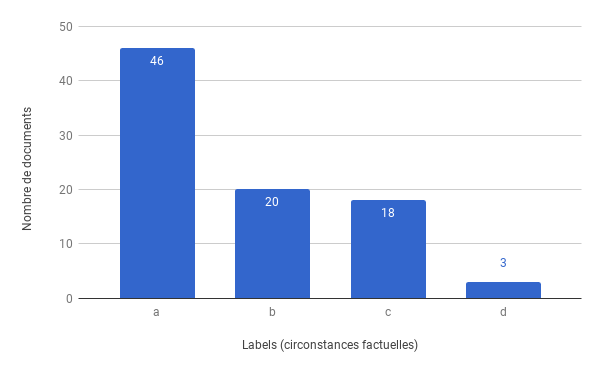
\includegraphics[scale=0.5]{arcpa-data-distrib.png}
%	\caption{Répartition des documents annotés par circonstances factuelles (\textit{arcpa}).}\label{fig:similarite:arcpa-data-distrib}
%\end{figure}

Les terminologies des cas se distinguent bien (Tableau \ref{tab:similarite:terminologie-resp_avocat}). Par conséquent, une représentation des documents qui mettrait en évidence de tels termes permettrait de retrouver les circonstances factuelles. 
\begin{table}[ht]
	\centering \scriptsize
	\begin{tabular}{|l|p{.85\textwidth}|}
		\hline
		\textbf{Corpus} & \textbf{Terminologie} \\ \hline
		\textit{arcpa} & chance, perte chance, avocat, perte, diligence, chance obtenir, perdre, client, devoir conseil, manquement
		\\ \hline
		\textit{cas a} & chance, perte chance, chance succès, perte, client, préjudice indemnisable, article code commerce, indemnisable, condamnation emporter, emporter nécessairement rejet
		\\ \hline
		\textit{cas b} & défense intérêt, intérêt client, avocat, contractuel égard, responsabilité contractuel droit, responsabilité professionnel avocat, contractuel droit commun, assurer défense intérêt, civil avocat, grief articuler
				\\ \hline
		\textit{cas c} & rédacteur acte, rédacteur, avocat rédacteur acte, avocat rédacteur, qualité rédacteur acte, rédaction acte, qualité rédacteur, projet acte, prendre initiative conseiller, initiative conseiller
		\\ \hline
		\textit{cas d} & revêtir aucun, revêtir aucun caractère, article code, article code procédure, faire référence aucun, fautif madame, civil profit autre, civil depuis, mention expresse, moyen dont
		\\ \hline
	\end{tabular}

	\textit{10 premiers termes lémmatisés de 1 à 3 mots sélectionnés à l'aide du coefficient de corrélation $ngl$ (cf. \ref{sec:quanta:poids-globaux-superv})}
	\caption{Terminologies de  la catégorie  $arcpa$ et de ses circonstances factuelles manuellement annotées.}\label{tab:similarite:terminologie-resp_avocat}
\end{table}

Pour l'évaluation non supervisée, les corpus des chapitres \ref{chap:quanta} et \ref{chap:sensresultat} sont aussi employés. Ils sont notés $\mathcal{D}_{acpa}$, $\mathcal{D}_{concdel}$, $\mathcal{D}_{danais}$,$\mathcal{D}_{dcppc}$, $\mathcal{D}_{doris}$, $\mathcal{D}_{styx}$.

\subsection{Protocole et outils logiciels}
La métrique apprise est entraînée sur une base générée, puis nous l'évaluons sur le corpus annoté $\mathcal{D}_{arcpa}$ restreint aux 74 documents n'appartenant qu'à l'un des cas $L = \lbrace a, b, c \rbrace$ (les chevauchements ne sont pas traités).  Les documents sont pré-traités avant leur représentation vectorielle. Ce pré-traitement consiste à les  sectionner (chapitre \ref{chap:structuration}), à les restreindre à la section Motifs, à mettre en minuscule et lemmatiser leur contenu, puis à y éliminer la ponctuation et des mots inutiles (\textit{stop words})  car ils sont généralement indépendants de toute catégorie. Après pré-traitement, les documents ont une taille allant de 208 à 3812 mots dont une moyenne de 1381 mots. Pour générer les données  d'entrainement de $Dis_M$, le vocabulaire $W$ utilisé est restreint aux mots du corpus original $D$ sur lequel il faut appliquer les catégorisations. La représentation vectorielle emploie des modèles de type TF-IDF (poids local $\times$ poids global $\times$ facteur de normalisation, cf. \ref{sec:quanta:classification}) avec des n-grammes de 1 à 3 mots. %Chaque poids global $g(t)$ d'un terme $t$ est multiplié par le logarithme du nombre de mots de $t$ donnant ainsi une nouvelle formulation $\hat{g}(t) = \log_2{\vert t \vert} \times g(t)$ qui, par conséquent, augmente le poids des longs termes qui sont rares mais parfois plus discriminants. 
Les poids globaux sont appris sur la discrimination entre deux corpus $\mathcal{D}_{c}$ et $\mathcal{D}_{\overline{c}}$ ($\setsize{\mathcal{D}_{\overline{arcpa}}} = 427$ documents) c'est-à-dire la terminologie d'une catégorie $c$ de demandes.

 La librairie Python Scikit-Learn \citep{Pedregosa2011scikit-learn} a été utilisée pour les implémentations des algorithmes de réduction de dimension, et ceux du DBSCAN, de la catégorisation spectrale (\textit{Spectral Clustering}), et du regroupement hiérarchique (\textit{Agglomerative Clustering}). Les implémentations des C-moyennes floues probabilistes (\textit{Probabilistic FCM}) et des arbres aléatoires (\textit{Random Forest}) proviennent respectivement des librairies \textit{scikit-cmeans 0.1}\footnote{\url{https://bm424.github.io/scikit-cmeans/index.html}} et RandomForestClustering\footnote{\url{https://github.com/joshloyal/RandomForestClustering/}}. La distance WMD est celle implémentée dans la librairie Gensim de \citet{rehurek2010gensim}. Les expérimentations utilisent un modèle de plongement lexical de type GLoVE  \citep{pennington2014glove} entraîné sur un corpus de +800k décisions de justice lémmatisées avec des fenêtres de contexte de 15 mots. Ce modèle dispose de 32445 mots représentés par des vecteurs de 300 dimensions. Le vecteur $\vec{t}$ d'un terme $t$ de $n$ mots $(w_1, w_2, \cdots, w_n)$ est obtenu en concaténant leur vecteur respectif de la droite vers la gauche: $\vec{t}=[\vec{w_1}\vec{w_2}\cdots \vec{w_n}]$.

\subsection{Validité de la distance apprise}
Pour la catégorie \textit{arcpa}, la base d'entraînement $B_\mathcal{M}$ comprend 935 documents dont 10 documents synthétiques générés pour chacun des 85 documents. Sur un modèle TF-IDF, la régression linéaire approxime bien la distance proposée $Dis_\mathcal{M}$ car elle a un faible taux d'erreur (Figure \ref{fig:similarite:eval-regression}).

%\begin{figure}[!htb]
% 	\centering 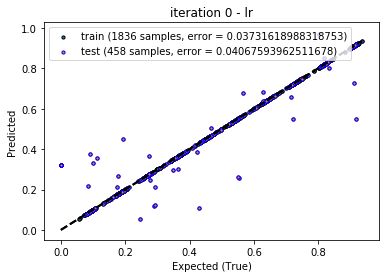
\includegraphics[width=0.5\textwidth]{eval-lr.png} \hfil
%	%\includegraphics[width=0.49\textwidth]{eval-mlp.png}
%	
%	\caption{Différence entre valeurs prédites et  attendues par la distance apprise}\label{fig:similarite:eval-regression}
%\end{figure}
%
%\begin{figure}[!htb]
%	\centering 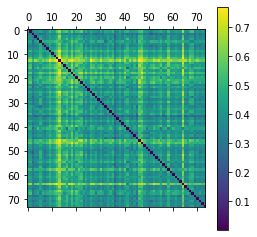
\includegraphics[scale=0.4]{distance_matrix.png}
%	\caption{Matrice des distances de la métrique apprise sur $\mathcal{D_{\text{arcpa}}}$}\label{fig:similarite:distance_matrix}
%\end{figure}
\begin{figure}[!htb]
\begin{subfigure}[ht]{0.49\textwidth}
	\centering 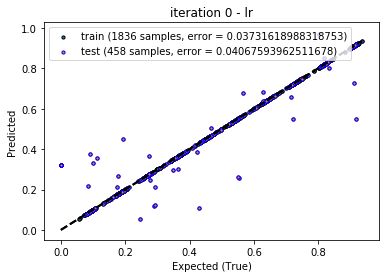
\includegraphics[width=\textwidth]{eval-lr.png} \hfil
	%\includegraphics[width=0.49\textwidth]{eval-mlp.png}
	
	\caption{Différence entre valeurs prédites et valeurs attendues}\label{fig:similarite:eval-regression}
\end{subfigure}
\begin{subfigure}[ht]{0.49\textwidth}
	\centering 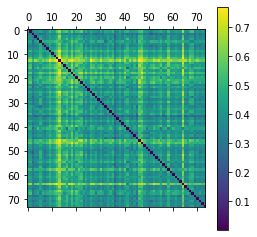
\includegraphics[scale=0.66]{distance_matrix.png}
	\caption{Matrice des distances entre documents}\label{fig:similarite:distance_matrix}
\end{subfigure}
\caption{Validité de la distance apprise.}
\end{figure}

D'après la matrice des distances entre les 74 documents de $\mathcal{D_{\text{arcpa}}}$ (Figure \ref{fig:similarite:distance_matrix}),  la "non-négativité", l'identité discernable, et la symétrie sont respectée car toutes les valeurs sont non-négative, seule la diagonale est nulle, et la matrice est symétrique. De plus, toutes les distances sont comprises entre 0 et 1, et par conséquent la métrique est normée.



L'inégalité triangulaire est vérifiée car $Dis_\mathcal{M}(d,d'') - (Dis_\mathcal{M}(d,d') + Dis_\mathcal{M}(d',d'')) \leq 0, \forall (
d,d',d'') \in \mathcal{D}_{arcpa} \times \mathcal{D}_{arcpa} \times \mathcal{D}_{arcpa}$ (Figure \ref{fig:similarite:matrice_inegalite_triangulaire}).

\begin{figure}[!htb]
	\centering 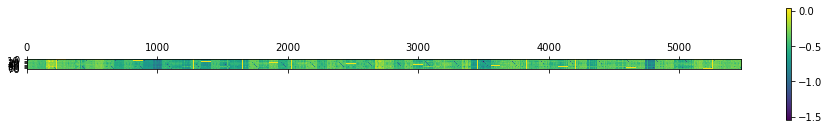
\includegraphics[width=0.8\textwidth]{inegalite_triangulaire.png}
	
	\scriptsize{$Dis_\mathcal{M}(d,d'') - (Dis_\mathcal{M}(d,d') + Dis_\mathcal{M}(d',d'')), \forall (d,d',d'') \in \mathcal{D}_{arcpa} \times \mathcal{D}_{arcpa} \times \mathcal{D}_{arcpa}$, avec les $d$ indicés en lignes et les paires $(d',d'')$ en colonnes.}
	\caption{Matrice de vérification de l'inégalité triangulaire}\label{fig:similarite:matrice_inegalite_triangulaire}
\end{figure}
 

\subsection{Sélection de la représentation optimale des textes}
\label{sec:similarite:select-repr-optimal}
En considérant la catégorisation manuelle de $\mathcal{D}_{arcpa}$, différentes représentation vectorielles peuvent être comparées, à l'aide de la silhouette, sur leur habilité à séparer les clusters manuels de documents dans l'espace. Nous comparons ici les combinaisons de différents poids locaux (Tableau \ref{tab:quanta:metriq_locales}), poids globaux (cf. \ref{sec:quanta:extract-terminologie-domaine}) et méthodes de réduction de dimensions (cf. \ref{sec:similarite:reduction-dimension}). 
Le Tableau \ref{tab:similarite:silhouette-vecteur-manuel} présente la représentation de largeur moyenne optimale de silhouette sur les données annotées pour chaque distance. Pour les réductions par ALD, ALS, et FNM, le nombre de thèmes est déterminé entre 4 et 10.

\begin{table}[!htb]
	\scriptsize \centering
	\begin{tabular}[pos]{|l|c|l|}
		\hline
		\textbf{Distance}&\textbf{Base$^a$}&\textbf{Silhouette optimale   (pondération, réduction, dim.)} \\ \hline
		$Dis_{jaccard}$ & 0.001 & 0.212 (TP-NGL, FNM, 4) \\ \hline
		$Dis_{cos}$ & 0.002 & 0.202 (TP-NGL, FNM, 4) \\ \hline
		$Dis_{M}$ & -0.049 & 0.195 (TP-NGL, FNM, 4) \\ \hline
		$Dis_{braycurtis}$ & 0.002& 0.182 (TP-NGL, FNM, 4) \\ \hline
		$Dis_{euclidienne}$ & 0.001& 0.168  (TP-NGL, FNM, 4) \\ \hline
		$Dis_{manhattan}$ & -0.019& 0.17   (TP-NGL, FNM, 4) \\ \hline
		$Dis_{pearson}$ & 0.014 & 0.057 (TP-CHI2, aucun, 19763) \\ \hline
		$Dis_{wmd}$ & -0.096 &  - \\ \hline
	\end{tabular}

	$^a$ occurrence de mots pour $Dis_{wmd}$, et TF-IDF pour les autres
    \caption{Meilleures représentations sur la catégorisation manuelle.} \label{tab:similarite:silhouette-vecteur-manuel}
\end{table}

 
Le modèle vectoriel TP-NGL réduit à 4 dimensions par la factorisation de matrice non négative (FNM) est préférée par la majorité des distances. Nous remarquons que la pondération globale supervisée (NGL et CHI2) met en évidence non seulement la terminologie de la catégorie de demande mais aussi celle des circonstances factuelles associées. La FNM marche mieux en moyenne pour toutes les classes avec des silhouettes maximales comprises entre 0.052 et 0.212, suivie de l'ALS (0.048 -- 0.119) et de l'ACP (0.029 -- 0.079). Les scores de silhouette maximales observés par l'ALD (-0.032 -- -0.001) sont moins bons que la représentation sans réduction (0.001 -- 0.008). La réduction par la méthode du barycentre des termes quant à elle donne un score de silhouette compris -0.048 et 0.013 au maximum sur l'ensemble des distances, avec une moyenne de 0.002.
Les représentations sélectionnées sont utilisées dans la suite. 

Le Tableau \ref{tab:similarite:silhouette-vecteur-manuel} classe aussi les distances en fonction de leur adaptabilité à la tâche, et la $Dis_\mathcal{M}$ se replace bien grâce à la représentation optimale. $Dis_{wmd}$ n'a pas été adaptée avec un modèle vectoriel plus adéquat que le sac-de-mots. Par conséquent, elle présente un score légèrement moins bon que celui d'un regroupement aléatoire (négatif et proche de 0).
\subsection{Catégorisation du corpus annotées manuellement}
\subsubsection{Nombre prédéfini de clusters}
 Le Tableau \ref{tab:similarite:validation-supervisee-k3} présente les mesures ARI, NMI et $F_1$-mesure de la catégorisation par K-moyennes et K-medoïdes sur $\mathcal{D}_{arcpa}$, avec $K=3$. 

\begin{table}[!htb]
	\centering \scriptsize
	\begin{tabular}[pos]{|l|l|c|c|c|c|c|c|}
		\hline
		\textbf{Distance}& \textbf{Algorithme}& \textbf{Silhouette}& \textbf{ARI} & \textbf{NMI} & \textbf{R} & \textbf{P} & \textbf{$F_1$} \\ \hline
		 $Dis_\mathcal{M}$          & K-moyennes    & 0.403      & 0.411 & 0.427 & 0.574  & 0.648     & \textbf{0.607} \\ \hline
		 $Dis_\mathcal{M}$          & K-medoïdes  & 0.398      & 0.321 & 0.340 & 0.483  & 0.591     & 0.532 \\ \hline
		 $Dis_{braycurtis}$ & K-moyennes    & 0.370      & 0.364 & 0.382 & 0.545  & 0.603     & 0.570 \\ \hline
		 $Dis_{braycurtis}$ & K-medoïdes  & 0.358      & 0.272 & 0.292 & 0.444  & 0.540     & 0.487 \\ \hline
		 $Dis_{cosine}$     & K-moyennes    & 0.422     & 0.389 & 0.406 & 0.556  & 0.616     & 0.583 \\ \hline
		 $Dis_{cosine}$     & K-medoïdes  & \textbf{0.448}      & 0.437 & \textbf{0.455} & 0.656  & 0.598     & \textbf{0.626} \\ \hline
		 $Dis_{euclidean}$  & K-moyennes    & 0.372      & \textbf{0.417} & \textbf{0.434} & 0.591  & 0.603     & 0.592 \\ \hline
		 $Dis_{euclidean}$  & K-medoïdes  & 0.369      & 0.392 & 0.409 & 0.566  & 0.672     & 0.615 \\ \hline
		 $Dis_{jaccard}$    & K-moyennes    & \textbf{0.442}      & 0.371 & 0.389 & 0.554  & 0.600     & 0.574 \\ \hline
		 $Dis_{jaccard}$    & K-medoïdes  & 0.431      & \textbf{0.440} & \textbf{0.455} & 0.529  & 0.645     & 0.581 \\ \hline
		 $Dis_{manhattan}$  & K-moyennes    & 0.390      & 0.376 & 0.394 & 0.567  & 0.582     & 0.571 \\ \hline
		 $Dis_{manhattan}$  & K-medoïdes  & -0.059     & 0.097 & 0.127 & 0.479  & 0.422     & 0.448 \\ \hline
		 $Dis_{pearson}$    & K-moyennes    & 0.434      & 0.088 & 0.117 & 0.585  & 0.487     & 0.530 \\ \hline
		 $Dis_{pearson}$    & K-medoïdes  & -0.019     & 0.111 & 0.136 & 0.421  & 0.476     & 0.447 \\ \hline
		 dis\_wmd    & K-medoïdes  & 0.105 & -0.004&	0.024&	0.333&	0.401&	0.364 \\ \hline
	\end{tabular}
	\caption{Evaluation de la catégorisation par K-moyennes et K-medoïdes sur $\mathcal{D}_{arcpa}$ avec le nombre de clusters prédéfini à $K=3$.} \label{tab:similarite:validation-supervisee-k3}
\end{table}

Les valeurs de silhouette se reflètent plus sur les indices ARI et NMI, mais moins sur la $F_1$-mesure. Suivant le score $F_1$, $Dis_M$, semble le mieux adaptée pour les K-moyennes, et $Dis_{cos}$ pour les K-medoïdes. Mais les distances, $Dis_{jaccard}$, $Dis_{cos}$, $Dis_{euclidienne}$ semblent faire le mieux le compromis entre les différents critères de validation.


\subsubsection{Nombre de clusters déterminé automatiquement}
Nous analysons ici  la détermination du nombre de cluster par la méthode de la silhouette pour chaque distance (Tableau \ref{tab:similarite:validation-supervisee-optKbySilhouette}). La sélection de $K$ est effectué pour les valeurs entre 2 et 30. Même si $Dis_\mathcal{M}$ retrouve le nombre attendu avec les K-moyennes, $4$ est la plus valeur la plus choisie par les distances, et 4 donne une $F_1$-mesure au maximum de 0.551 et un ARI de 0.398 avec $Dis_{cos}$. Les valeurs déterminées (entre 2 et 6) sont très proches de la valeur attendue 3 pour toutes les distances.  Notons aussi que l'efficacité de $Dis_\mathcal{M}$ et $Dis_{cos}$ reste presque aussi élevée qu'avec un $K$ prédéfini (Tableau \ref{tab:similarite:validation-supervisee-k3}). $Dis_\mathcal{M}$ et $Dis_{cos}$ semblent ainsi former de bonnes combinaison avec respectivement les K-moyennes et les K-medoïdes. Par ailleurs, seules $Dis_{manhattan}$ et $Dis_{wmd}$ obtiennent de très faibles valeurs pour les indices ARI et NMI. Même si ces valeurs sont inférieures pour les autres distances, ces dernières, en particulier $Dis_\mathcal{M}$, $Dis_{jaccard}$ et $Dis_{cos}$, parviennent quand même à un bon compromis entre les 3 critères ARI, NMI et $F_1$. $Dis_{jaccard}$ et $Dis_{cos}$ sont efficaces autant avec les K-moyennes qu'avec les K-medoïdes. Elles parviennent à associer une bonne validation non-supervisée (silhouette) à une bonne validation non-supervisée.

\begin{table}[!htb]
	\centering \scriptsize
	\begin{tabular}[pos]{|l|l|c|c|c|c|c|c|c|}
		\hline
		\textbf{Distance}& \textbf{Algorithme}& \textbf{K}& \textbf{Silhouette}& \textbf{ARI} & \textbf{NMI} & \textbf{R} & \textbf{P} & \textbf{$F_1$} \\ \hline
		$Dis_\mathcal{M}$          & K-moyennes    & \textbf{3} & 0.438      & \textbf{0.407} & \textbf{0.423} & 0.552  & 0.654     & \textbf{0.599} \\ \hline
		$Dis_\mathcal{M}$          & K-medoïdes  & 6 & 0.453      & 0.359 & 0.395 & 0.298  & 0.669     & 0.413 \\ \hline
		$Dis_{braycurtis}$ & K-moyennes    & 4 & 0.473      & 0.383 & 0.407 & 0.446  & 0.658     & 0.532 \\ \hline
		$Dis_{braycurtis}$ & K-medoïdes  & 5 & 0.448      & 0.344 & 0.375 & 0.331  & 0.645     & 0.437 \\ \hline
		$Dis_{cosine}$     & K-moyennes    & 4 & 0.528      & 0.383 & 0.407 & 0.446  & 0.658     & 0.532 \\ \hline
		$Dis_{cosine}$     & K-medoïdes  & 4 & 0.526      & \textbf{0.398} & \textbf{0.421} & 0.464  & 0.680     & \textbf{0.551} \\ \hline
		$Dis_{euclidean}$  & K-moyennes    & 5 & 0.478      & 0.365 & 0.395 & 0.341  & 0.670     & 0.452 \\ \hline
		$Dis_{euclidean}$  & K-medoïdes  & 5 & 0.456      & 0.313 & 0.346 & 0.335  & 0.619     & 0.434 \\ \hline
		$Dis_{jaccard}$    & K-moyennes    & 4 & 0.570      & 0.367 & 0.391 & 0.439  & 0.643     & 0.522 \\ \hline
		$Dis_{jaccard}$    & K-medoïdes  & 4 & \textbf{0.560}      & 0.389 & 0.412 & 0.451  & 0.666     & 0.538 \\ \hline
		$Dis_{manhattan}$  & K-moyennes    & 4 & 0.482      & 0.376 & 0.400 & 0.452  & 0.657     & 0.535 \\ \hline
		$Dis_{manhattan}$  & K-medoïdes  & 5 & 0.452      & 0.368 & 0.397 & 0.345  & 0.675     & 0.456 \\ \hline
		$Dis_{pearson}$    & K-moyennes    & 2 & \textbf{0.611}      & 0.054 & 0.072 & 0.746  & 0.453     & 0.564 \\ \hline
		$Dis_{pearson}$    & K-medoïdes  & 2 & 0.171      & 0.152 & 0.166 & 0.598  & 0.482     & 0.534 \\ \hline
		$Dis_{wmd}$      & K-medoïdes  & 2 & 0.332      & -0.016 & 0.002 & 0.545  & 0.397     & 0.459 \\ \hline
	\end{tabular}
	\caption{Evaluation de la catégorisation par K-moyennes et K-medoïdes sur $\mathcal{D}_{arcpa}$ avec détermination du nombre de clusters avec la silhouette.} \label{tab:similarite:validation-supervisee-optKbySilhouette}
\end{table}

La Figure \ref{fig:similarite:optimalK_with_silhouette_kmeans_dis_m_K2-30} montre l'évolution de la valeur de la silhouette en fonction du nombre de clusters pour $Dis_\mathcal{M}$ utilisé dans les K-moyennes. 

\begin{figure}[!htb]
	\centering 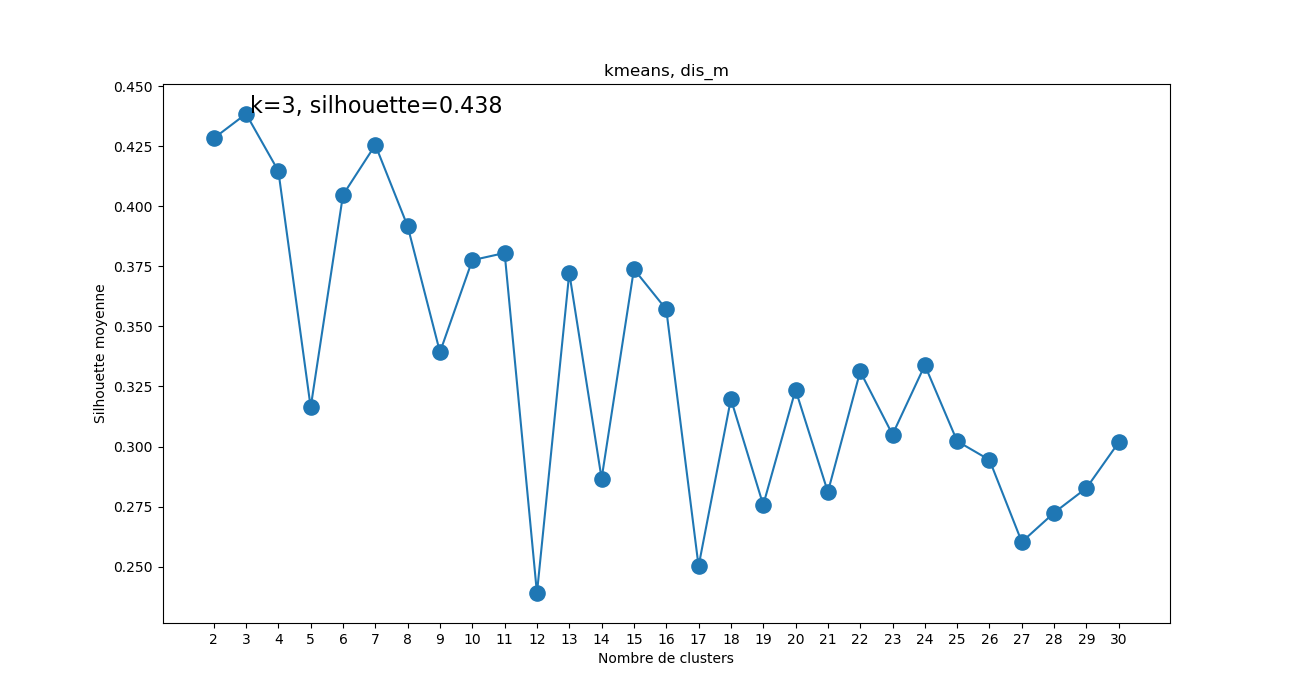
\includegraphics[width=0.6\textwidth]{optimalK_with_silhouette_kmeans_dis_m_K2-30.png} \hfil
	%\includegraphics[width=0.49\textwidth]{eval-mlp.png}
	
	\caption{Evolution de la silhouette pour les K-moyennes et la distance apprise.}\label{fig:similarite:optimalK_with_silhouette_kmeans_dis_m_K2-30}
\end{figure}
 

\subsubsection{Autres algorithmes de catégorisation}
Avec la représentation sélectionnée TP-NGL, nous appliquons d'autres algorithmes de catégorisation sur $\mathcal{D}_{arcpa}$ (Tableau \ref{tab:similarite:validation-supervisee-optKbySilhouette-autres_algos}). L'algorithme de regroupement à chevauchements des C-moyennes floues probabilistes (\textit{Probabilistic FCM}) est utilisé pour partitionner le corpus en choisissant un seul cluster pour chaque document (celui pour qui le degré d'appartenance est maximal). Seules le regroupement hiérarchique et les C-moyennes floues probabilistes parviennent à trouver un nombre de clusters (4) assez proche de ce celui attendu (3). Les forêts aléatoires ont une très basse $F_1$-mesure du fait du grand nombre de clusters déterminé. Par ailleurs, la tâche ne semble pas correspondre ni à  la catégorisation par densité qui tend toujours à mettre tous les documents dans un même cluster, ni à la catégorisation spectrale qui sélectionne un très grands nombre de clusters. 
\begin{table}[!htb]
	\centering \scriptsize
	\begin{tabular}[pos]{|l|c|c|c|c|c|c|c|}
		\hline
		\textbf{Algorithme}& \textbf{K}& \textbf{Silhouette}& \textbf{ARI} & \textbf{NMI} & \textbf{R} & \textbf{P} & \textbf{$F_1$} \\ \hline
		Spectral Clustering & 19 & 0.352 & 0.193 & 0.317 & 0.069 & 0.632 & 0.124 \\ \hline 
		DBSCAN & 2 & -1.000 & 0.000 & 0.000 & 1.000 & 0.398 & 0.570 \\ \hline 
		%K-moyennes & 4 & 0.524 & 0.383 & 0.407 & 0.446 & 0.658 & 0.532 \\ \hline 
		Agglomerative Clustering & 4 & 0.475 & 0.355 & 0.381 & 0.428 & 0.567 & 0.487 \\ \hline 
		Probabilistic FCM & 4 & 0.521 & 0.394 & 0.417 & 0.444 & 0.657 & 0.530 \\ \hline 
		Random Forest & 11 & 0.272 & 0.228 & 0.303 & 0.127 & 0.598 & 0.210 \\ \hline 
	\end{tabular}
	\caption{Evaluation de la catégorisation par d'autres algorithmes sur $\mathcal{D}_{arcpa}$ avec détermination du nombre de clusters avec la silhouette.} \label{tab:similarite:validation-supervisee-optKbySilhouette-autres_algos}
\end{table}

Le score de silhouette des C-moyennes floues probabilistes (Figure \ref{fig:similarite:optimalK_with_silhouette_ProbabilisticFuzzyCMeans_K2-30}) a une décroissance plus rapide et plus monotone que notre implémentation des K-moyennes (Figure \ref{fig:similarite:optimalK_with_silhouette_kmeans_dis_m_K2-30}).

\begin{figure}[!htb]
	\centering 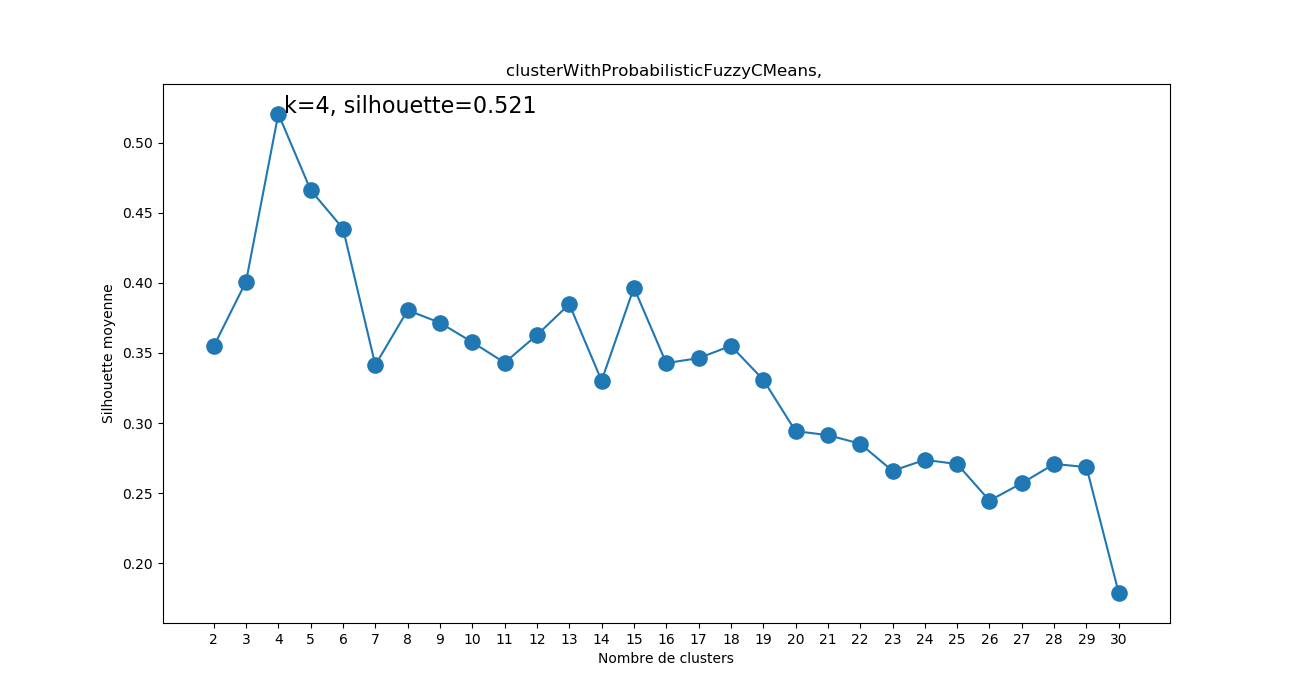
\includegraphics[width=0.6\textwidth]{optimalK_with_silhouette_ProbabilisticFuzzyCMeans_K2-30.png} \hfil
	%\includegraphics[width=0.49\textwidth]{eval-mlp.png}
	
	\caption{Évolution de la silhouette pour les C-moyennes floues probabilistes}\label{fig:similarite:optimalK_with_silhouette_ProbabilisticFuzzyCMeans_K2-30}
\end{figure}

\subsection{Catégorisation des corpus non annotés manuellement}
Les matrices document-terme des autres catégories sont construites à base la  représentation (TP-NGL, FMN,  4 thématiques) sélectionnée sur la catégorisation manuel (cf. \ref{sec:similarite:select-repr-optimal}). Le tableau \ref{tab:similarite:validation-nonsupervisee} présente les valeurs de silhouette ($\bar{s}_K$) obtenues par le K-moyennes et le k-medoid sur ces matrices. Les nombres déterminés de clusters restent bas (entre 2 et 6) malgré le fait qu'ils soient sélectionnés entre 2 et 30. 
\newlength{\mrcell}
\setlength{\mrcell}{0.8cm}
\begin{table}[!htb]
	\scriptsize
	\begin{subfigure}[ht]{0.49\textwidth}
	\begin{tabular}[pos]{|l|l|l|c|c|}
		\hline
		$\mathcal{D}$& \textbf{Distance} & \textbf{Algorithme}& \textbf{K}  & $\bar{s}_K$  \\ \hline
	\multirow{6}{\mrcell}{$\mathcal{D}_{acpa}$ (21$^*$)} & $Dis_\mathcal{M}$ & K-medoïdes & 2 & 0.769  \\ \cline{2-5}
	& $Dis_\mathcal{M}$ & K-moyennes & 2 & 0.769 \\ \cline{2-5}
	& $Dis_{cosine}$ & K-medoïdes & 5 & 0.694 \\ \cline{2-5}
	& $Dis_{cosine}$ & K-moyennes & 3 & 0.762  \\ \cline{2-5}
	& $Dis_{jaccard}$ & K-medoïdes & 2 & 0.499  \\ \cline{2-5}
	& $Dis_{jaccard}$ & K-moyennes & 3 & 0.769 \\ \hline
	\multirow{6}{\mrcell}{$\mathcal{D}_{concdel}$ (30)}  & $Dis_\mathcal{M}$ & K-medoïdes & 4 & 0.639  \\ \cline{2-5}
	& $Dis_\mathcal{M}$ & K-moyennes & 4 & 0.624  \\ \cline{2-5}
	& $Dis_{cosine}$ & K-medoïdes & 4 & 0.675  \\ \cline{2-5}
	& $Dis_{cosine}$ & K-moyennes & 4 & 0.632  \\ \cline{2-5}
	& $Dis_{jaccard}$ & K-medoïdes & 5 & 0.719  \\ \cline{2-5}
	& $Dis_{jaccard}$ & K-moyennes & 5 & 0.702\\ \hline
	\multirow{6}{\mrcell}{$\mathcal{D}_{danais}$ (198)} 
	& $Dis_\mathcal{M}$ & K-medoïdes & 4 & 0.403  \\ \cline{2-5}
	& $Dis_\mathcal{M}$ & K-moyennes & 2 & 0.442  \\ \cline{2-5}
	& $Dis_{cosine}$ & K-medoïdes & 4 & 0.475 \\ \cline{2-5}
	& $Dis_{cosine}$ & K-moyennes & 4 & 0.471  \\ \cline{2-5}
	& $Dis_{jaccard}$ & K-medoïdes & 3 & 0.483 \\ \cline{2-5}
	& $Dis_{jaccard}$ & K-moyennes & 3 & 0.482 \\ \hline
\end{tabular}
	\end{subfigure}
	\begin{subfigure}[ht]{0.49\textwidth}
		\begin{tabular}[pos]{|l|l|l|c|c|}
			\hline
			$\mathcal{D}$& \textbf{Distance} & \textbf{Algorithme}& \textbf{K}  & $\bar{s}_K$ \\ \hline
	\multirow{6}{\mrcell}{$\mathcal{D}_{dcppc}$ (91)} & $Dis_\mathcal{M}$ & K-medoïdes & 2 & 0.451  \\ \cline{2-5}
	& $Dis_\mathcal{M}$  & K-moyennes & 2 & 0.781  \\ \cline{2-5}
	& $Dis_{cosine}$ & K-medoïdes & 2 & 0.549 \\ \cline{2-5}
	& $Dis_{cosine}$ & K-moyennes & 2 & 0.925 \\ \cline{2-5}
	& $Dis_{jaccard}$ & K-medoïdes & 2 & -0.016  \\ \cline{2-5}
	& $Dis_{jaccard}$ & K-moyennes & 3 & 0.820 \\ \hline
	\multirow{6}{\mrcell}{$\mathcal{D}_{doris}$ (59)}  & $Dis_\mathcal{M}$ & K-medoïdes & 2 & 0.509  \\ \cline{2-5}
	& $Dis_\mathcal{M}$ & K-moyennes & 3 & 0.527  \\ \cline{2-5}
	& $Dis_{cosine}$ & K-medoïdes & 5 & 0.549 \\ \cline{2-5}
	& $Dis_{cosine}$ & K-moyennes & 4 & 0.586 \\ \cline{2-5}
	& $Dis_{jaccard}$ & K-medoïdes & 3 & 0.600 \\ \cline{2-5}
	& $Dis_{jaccard}$ & K-moyennes & 4 & 0.645 
	\\ \hline
	\multirow{6}{\mrcell}{$\mathcal{D}_{styx}$ (50)}  & $Dis_\mathcal{M}$ & K-medoïdes & 2 & 0.669 \\ \cline{2-5}
	& $Dis_\mathcal{M}$ & K-moyennes & 2 & 0.669 \\ \cline{2-5}
	& $Dis_{cosine}$ & K-medoïdes & 5 & 0.695 \\ \cline{2-5}
	& $Dis_{cosine}$ & K-moyennes & 4 & 0.705 \\ \cline{2-5}
	& $Dis_{jaccard}$ & K-medoïdes & 6 & 0.635 \\ \cline{2-5}
	& $Dis_{jaccard}$  & K-moyennes & 4 & 0.690 \\ \hline
	\end{tabular}
	\end{subfigure}

	$^*$ Nombre de documents
	
$\bar{s}_K$: largeur moyenne de la silhouette

	\caption{Evaluation non-supervisée des K-moyennes et K-medoïdes sur $\mathcal{D}_{acpa}, \mathcal{D}_{concdel}, \mathcal{D}_{danais}, \mathcal{D}_{dcppc}, \mathcal{D}_{doris}, \mathcal{D}_{styx}$.} \label{tab:similarite:validation-nonsupervisee}
\end{table}

La silhouette étant bonne en générale, on s'attend à ce que les groupes soient en majorité formés effectivement de décisions partageant les mêmes circonstances factuelles. Il est possible de se faire une idée des circonstances factuelles découvertes en observant leur terminologie qu'on peut extraire à l'aide d'une pondération globale supervisée comme le coefficient NGL. Considérons par exemple le regroupement avec les K-medoïdes combinés à la distance cosinus qui marche assez bien sur $\mathcal{D}_{arcpa}$. Pour la catégorie CONCDEL\footnote{CONDEL: dommages-intérêts pour concurrence déloyale}, on obtient 4 circonstances factuelles dont les champs lexicaux (Tableau \ref{tab:similarite:terminologie-clusters-concdel}) semblent définir les cas de contrefaçon pour le cluster 0, de publicité déloyale pour le cluster 1, de recrutement d'un salarié par un concurrent pour le cluster 2, et de contrats avec des partenaires pour le dernier cluster.


%\subsection{Terminologie des clusters générés}

\begin{table}[ht]
	\centering \scriptsize
	\begin{tabular}{|l|p{.85\textwidth}|}
		\hline
		\textbf{Cluster} & \textbf{Terminologie} \\ \hline
		\textit{0} & distinctif, reproduire, code propriété intellectuel, contrefaçon, attaque, dépôt marque, circonstance intervenir, intervenir jugement, intervenir jugement déférer, caractère distinctif
		\\ \hline
		\textit{1} & publicitaire, action concurrence, défaut qualité agir, action concurrence déloyal, qualité agir, fichier client, force chose juger, fonder demande titre, date transfert, celui -ci fonder
		\\ \hline
		\textit{2} & acte concurrence, acte concurrence déloyal, clause non concurrence, non concurrence, clause non, entreprise concurrent, démarchage, démarcher, salarié, massif
		\\ \hline
		\textit{3} & non concurrencer, clause non concurrencer, tout droit, résilier contrat, marcher, préjudice invoquer, détournement, compte entre partie, contrat @card@ juillet, compte entre
		\\ \hline
	\end{tabular}
	
	\textit{10 premiers termes de 1 à 3 mots sélectionnés à l'aide du coefficient de corrélation $ngl$ (cf. \ref{sec:quanta:poids-globaux-superv})}
	\caption{Terminologies des circonstances factuelles découvertes en combinant les K-medoïdes et la distance cosinus sur $\mathcal{D}_{concdel}$.}\label{tab:similarite:terminologie-clusters-concdel}
\end{table}

Pour la catégorie DORIS\footnote{DORIS: dommages-intérêts pour trouble anormal de voisinage},  on obtient 5 circonstances factuelles dont les champs lexicaux (Tableau \ref{tab:similarite:terminologie-clusters-doris}) semblent définir les cas d'excès de trouble pour le cluster 0, de différents entre copropriétaires d'un immeuble pour le cluster 1, de toit dépassant la limite entre deux habitations pour le cluster 2, et d'ouvrage dépassant la hauteur limite autorisée pour le dernier cluster. Le cluster 3 est plus difficile à interpréter  même s'il semble s'agir du droit de jouir d'une propriété.

\begin{table}[ht]
	\centering \scriptsize
	\begin{tabular}{|l|p{.85\textwidth}|}
		\hline
		\textbf{Cluster} & \textbf{Terminologie} \\ \hline
		\textit{0} & excéder inconvénient, inconvénient normal, excéder inconvénient normal, normal voisinage, inconvénient normal voisinage, inconvénient, trouble excéder inconvénient, trouble excéder, excéder, normal
		\\ \hline
		\textit{1} & copropriétaire, syndicat copropriétaire, syndicat, condamner in, anormal voisinage, trouble anormal voisinage, in, trouble anormal, syndic, jouissance subir
		\\ \hline
		\textit{2} & deux fond|fonds, séparatif deux fond|fonds, limite séparatif deux, ordonner démolition, séparatif deux, implanter, condamner démolir, devoir établir toit, devoir établir, toit manière
		\\ \hline
		\textit{3} & manière plus, chose manière plus, chose manière, usage prohiber loi, prohiber loi règlement, prohiber loi, absolu, usage prohiber, manière plus absolu, plus absolu, 
		\\ \hline
		\textit{4} & situer zone, hauteur @card@ mètre, hauteur dépasser, appel contester, vitrer, dont hauteur dépasser, urbaniser, recevabilité <unknown> appel, cahier charge lotissement, charge lotissement, 
		\\ \hline
	\end{tabular}
	
	\textit{10 premiers termes de 1 à 3 mots sélectionnés à l'aide du coefficient de corrélation $ngl$ (cf. \ref{sec:quanta:poids-globaux-superv})}
	\caption{Terminologies des circonstances factuelles découvertes en combinant les K-medoïdes et la distance cosinus sur $\mathcal{D}_{doris}$.}\label{tab:similarite:terminologie-clusters-doris}
\end{table}


%\begin{tabular}[pos]{|l|l|c|c|}
%	\hline
%	\textbf{Corpus}& \textbf{Distance}& \textbf{K} & \textbf{S}  \\ \hline
%	\multirow{2}{*}{$\mathcal{D}_{acpa}$ (21$^*$)} & $Dis_{cos}$  & 3 & 0.525 \\ \cline{2-4}
%	& $Dis_{M}$ & 2 & 0.770\\ \hline
%	\multirow{2}{*}{$\mathcal{D}_{concdel}$ (30)}  & $Dis_{cos}$  & 4 & 0.697  \\ \cline{2-4}
%	& $Dis_{M}$ & 4 & 0.652\\ \hline
%	\multirow{2}{*}{$\mathcal{D}_{danais}$ (198)}  & $Dis_{cos}$  & 5 & 0.426 \\ \cline{2-4}
%	& $Dis_{M}$ & 4 & 0.403\\ \hline
%	\multirow{2}{*}{$\mathcal{D}_{dcppc}$ (91)}  & $Dis_{cos}$  &  2 & 0.549 \\ \cline{2-4}
%	& $Dis_{M}$ &2 & 0.451\\ \hline
%	\multirow{2}{*}{$\mathcal{D}_{doris}$ (59)}  & $Dis_{cos}$  & 5 & 0.549 \\ \cline{2-4}
%	& $Dis_{M}$ & 2 & 0.509\\ \hline
%	\multirow{2}{*}{$\mathcal{D}_{styx}$ (50)}  & $Dis_{cos}$  & 4 & 0.572 \\ \cline{2-4}
%	& $Dis_{M}$ &2 & 0.694\\ \hline
%\end{tabular}
\section{Conclusion}
\label{sec:similarite:conclusion}
Les circonstances factuelles organisent les décisions d'une même catégorie de demande mais sont illimitées car elles correspondent aux faits courants de la vie. Leur découverte est indispensable afin de rapprocher les litiges non décidés des cas similaires de la jurisprudence.  Ce chapitre aborde ce problème comme une tâche de catégorisation non supervisée de documents. La proposition faite ici est double: (i) l'apprentissage d'une métrique de dis-similarité en considérant qu'un document est obtenu par transformation de tout autre document, (ii) l'exploitation de la faible quantité de catégorisations manuelles  pour sélectionner la représentation de texte qui correspond au mieux à la sémantique des circonstances factuelles. Le schéma sélectionné permet de transformer de nouveaux corpus non annotés afin d'y découvrir les circonstances factuelles par catégorisation non supervisée. Les expérimentations montrent une amélioration considérable par rapport au modèle de base TF-IDF. La silhouette reste néanmoins faible. Ce qui signifie que la réduction de dimension par FNM est efficace mais il faudrait la combiner avec de meilleurs modèles vectoriels ou mieux l'intégrer au processus de catégorisation comme le font \citet{xie2013MGCTM} avec l'allocation latente de Dirichlet. Néanmoins cette sélection de représentation permet d'obtenir une assez bonne efficacité de catégorisation sur le corpus annoté. En effet, nous obtenons, avec respectivement les K-moyennes et les K-medoïdes, 0.599 et 0.551 de $F_1$-mesure, correspondant à 0.407 et 0.398 de ARI, et 0.423 et 0.421 de NMI pour un nombre de clusters déterminé automatiquement. Ces résultats se traduisent aussi sur la largeur moyenne de la silhouette autant pour le corpus annoté (0.438 et 0.526 respectivement) que pour les six corpus non annotés utilisés (entre 0.403 et 0.770 au max pour toutes les catégories). La métrique apprise s'accorde mieux avec les K-moyennes que les autres distances selon différents indices de validation, et même pour la détermination du nombre de clusters.

Dans ce chapitre, la représentation vectorielle n'est sélectionnée que sur un seul corpus. Il serait intéressant à l'avenir d'annoter plusieurs corpus pour sélectionner la représentation qui correspond le mieux en moyenne aux circonstances factuelles sur l'ensemble de ces catégorisations manuelles. De plus, les expérimentations doivent être étendues au regroupement à chevauchement pour les affaires  concernant plus d'une circonstance factuelle.